\documentclass[en,license=none]{../../../eplsummary}
\usepackage{../../../eplcode}

\usepackage{esdiff}

\usepackage{color}
\usepackage{mathtools}
\usepackage{wrapfig}

\DeclareMathOperator*{\plim}{plim}

%to display a warning sign (code from https://tex.stackexchange.com/a/159701)
\usepackage{newunicodechar}
\newcommand\warn{%
 \makebox[1.2em][c]{%
 \makebox[0pt][c]{\raisebox{.1em}{\tiny!}}%
 \makebox[0pt][c]{\color{red}$\bigtriangleup$}}}%

\hypertitle{Machine Learning : regression dimensionality reduction and data visualization}{7}{ELEC}{2870}
{Guillaume Derval\and Benoît Legat \and Valentin Lemaire \and Gauthier de Moffarts \and Brieuc de Voghel \and Séverine Mersch-Mersch}
{Michel Verleysen and John Lee}

\newcommand{\ex}[1]{\\ • exemple: #1}
\newcommand{\newpar}{\vspace{\baselineskip} \noindent}

\section{Introduction}
    \subsection{What is machine learning}
    
    The role of machine learning is to build a machine that learns a model from the data.
    In statistics, one often supposes that the data follow a certain distribution and try to approximate the value of those parameters. 
    On the other hand, in machine learning we try to make the least amount of assumption on the data
    to let enough degrees of freedom for the machine to learn a good model.
    
    Machine Learning can be decomposed in 5 steps,
    only the last 3 are covered in this course:
    \begin{enumerate}
    	\item
    	      Preprocessing
    	\item
    	      Feature generation
    	\item
    	      Feature selection (Section~\ref{sec:featuresel})
    	\item
    	      Model generation (Section~\ref{sec:modelgen})
    	\item
    	      Validation
    \end{enumerate}
    
    \subsection{History}
    \begin{center}
    	\begin{tabular}{lll}
    		1940--1965 & Hebb                                 & Biological learning rule                          \\
    		           & McCulloch \& Pitts                   & Binary decision units                             \\
    		           & Rosenblatt                           & Perceptron, learning                              \\
    		1969       & Minsky \& Papert                     & Limits to Perceptron                              \\
    		1974       & Werbos                               & Back-propagation                                  \\
    		1980s      & Hopfield                             & Recurrent networks                                \\
    		           & Parker, LeCun, Rumelhart, McClelland & Back-propagation                                  \\
    		           & Kohonen                              & Self-Organizing Maps                              \\
    		1990s      & Vapnik                               & Support Vector Machines                           \\
    		           & Many                                 & Feature selection, model selection, evaluation...
    	\end{tabular}
    \end{center}
    
    \subsection{Overfitting}
    How to detect overfitting:
    \begin{itemize}
    	\item by ploting a projection (hard)
    	\item by looking at the errors of the training set and test set. If they are very different, the model overfits.
    	\item by looking at the model parameters. They are usually large when it overfits.
    \end{itemize}
    
    Having a few sample or a large model order increases the risk of overfitting.
    
    We can limit this risk by using {\color{blue} regularization} in addition to the MSE (mean of squared errors):
    $$
    	\tilde{E}(\mathbf{w})=\frac{1}{N} \sum_{n=1}^{N}\left\{y\left(x_{n}, \mathbf{w}\right)-t_{n}\right\}^{2}{\color{blue} +\frac{\lambda}{N}\|\mathbf{w}\|^{2}}
    $$
    
    \subsection{Curse of dimensionality}
        % trying to write a better explanation
        % https://www.mygreatlearning.com/blog/understanding-curse-of-dimensionality/
    % \subsubsection{Problem}
    %     \paragraph{} The quantity of data needed increases exponentially with the number of features (dimensions). 
    %     \paragraph{} With 2 features (young-old and male-female) a population can be divided into 4 groups (young males, young females, ...). When increasing the number of features (adding rich-poor for example), the number of groups is multiplied (8 groups : young rich males, young poor males, ...).
    %     \paragraph{Data Sparsity} When the training samples are missing some of the combinations of features.
    %     \paragraph{Distance Concentration}
    % \subsubsection{Dimensionality reduction techniques}
    %     \paragraph{} 
        
    
    % old explanation
    % \subsubsection{Data sparsity}
    We need at least as much examples (data) as dimensions.
    If we cut each dimension by $x$, you have $x^n$ data samples.
    We need at least some data in each region.
    It increases exponentially.
    So we need feature selection!
    
    All our algorithms are sensitive to this problem, just differently.
    \subsection{Supervised learning}
    Building an in-out relation thanks to data with know desired output (label, value, etc.).
    It is used for \textbf{classification} and \textbf{regression} problems.
    \subsection{Unsupervised learning}
    Extracting some useful information from data without supplementary knowledge.
    It is used for \textbf{clustering}, \textbf{adaptive filtering}, and \textbf{visualization} problems.

\section{Principal Component Analysis (PCA)}
    Suppose the features are stored by rows in $X$
    and each column represents a sample. The goal of PCA is to find a new coordinate system where variables are decorrelated or even white (using a linear transformation of data $Y = WX$ and to reduce the number of variables in the new coordinate system to minimize the loss of information when backprojecting to the initial coordinate system.
    \subsection{Background}
        \paragraph{Moments} $\mu_X = \mathbb{E}_X[X^n] = \int_{-\infty}^\infty x^n f_X(x) dx$. 1st order moment is the expectation of a Random Variable, second-order central moment is the variance.
        Standard Deviation is $$\sigma_X = \sqrt{\mathbb{E}_X[(X-\mu_X)^2]}$$
        \paragraph{Covariance and Correlation} 
        $$C_{X,Y} = Cov[X_i, X_j] = \mathbb{E}_X[(X_i - \mu_{X_i})(X_j - \mu_{X_j})] = \mathbb{E}[X_iX_j] - \mathbb{E}_{X_i}[X_i] \mathbb{E}_{X_j}[X_j]$$
        $$Cor[X_i, X_j] = \frac{Cov[X_i, X_j]}{\sigma_{X_i}\sigma_{X_j}}$$
        Correlation coefficient r ($\in [-1, 1]$) tells us how well a regression line fits the data. A null correlation coefficient means there is no \textbf{linear} relationship between x and y.
        \paragraph{Statistical Independence} Having all elements of x independent means that : 
        $$f_X(X) = \prod_{i=1}^M f_{X_i}(x_i)$$
        Which means the covariance matrix is diagonal ($\mathbb{E}_X[X_i, X_j] = \mathbb{E}_{X_i}[X_i]\mathbb{E}_{X_j}[X_j]$ for $i \neq j$. It is a sufficient condition to get a diagonal covariance but not necessary.
    	\paragraph{Decorrelated}: Data $(X,Y)$ are decorrelated iff $C_{X,Y}$ is in the form of $\begin{pmatrix}
    			      \sigma_X^2 & 0          \\
    			      0          & \sigma_Y^2
    		      \end{pmatrix}$ (diagonal).
    	      The covariance of $N$ variables is computed using resp. $C_X = XX^\Tr / N$.
    	\paragraph{Whiteness}: Data $(X,Y)$ is white iff $C_{X,Y}$ is the identity matrix (and $\bar{X}=\bar{Y}=0$).
    	\paragraph{Sample Mean and Covariance}
    	Since Data are sampled from a Random Vector: $X = [x_k]_{1\leq k \leq N}$, we have:
    	$$\mathbb{E}_X[g(x)] \approx \sum_{k=1}^N g(x_k)f_X(x_k) \approx \frac{1}{N}\sum_{k=1}^N g(x_k)$$
    	Which implies:
        $$\hat{\mu}_{X_i} = \frac{1}{N}\sum_{k=1}^N x_{ik} \approx \mathbb{E}_X[X_i] = \mathbb{E}_{X_i}[X_i]$$ 
        And (with $1 = [1 ... 1]^\Tr$) $$\hat{\mu}_X = \left[\frac{1}{N}\sum_{k=1}^N x_{ik}\right]_{1 \leq i \leq N} = \frac{1}{N} X1$$\\
        In the same way: $$\hat{\Sigma}_X = \left[\frac{1}{N}\sum_{k=1}^N(x_{ik}- \hat{\mu}_{X_i})(x_{jk}- \hat{\mu}_{X_j})\right]_{1\leq i, j \leq N} = \frac{1}{N} (XC)(XC)^\Tr = \frac{1}{N} XCCX^\Tr $$\\
        Where $C = I - \frac{1}{N}1 1^\Tr$ is the centering matrix.
        
        \paragraph{Positive Semi Definiteness (PSD)} A square, symmetric matrix A is positive semi definite (PSD) iff $x^\Tr A x \geq 0$ for every non-zero column vector $x$. It is noted : $A \succeq 0$. A covariance matrix is always PSD as any matrix $A$ that can be written in the form $A = BB^\Tr$ is PSD.
        
        \paragraph{Orhtogonal matrices} U is orthogonal iff $U^\Tr U = I = UU^\Tr$. It implies $U^{-1} = U^\Tr$. The columns of $U$ are perpendicular to each other and have unit length.
    	
    	\paragraph{Eigenvalue Decomposition (EVD)}
    	If a matrix $A$ is square, symmetric and real-valued, it can be written as : $A = V \Lambda V^\Tr = \sum_{i=1}^M \lambda_i v_i v_i^\Tr$ with $V$ orhtogonal and $\Lambda$ diagonal. The columns of $V$ are eigenvectors and the elements of $\Lambda$ are eigenvalues. Since $C_X$ is PSD :  $C_X = V \Lambda V^\Tr$ with $\lambda_i \geq 0 \;\;\forall i$\\
    	
    	Since the relation is linear, eigenvalues and vectors can be switched in any order, convention is to sort them in descending order of eigenvalues (eigenvalues and vectors must be in the same order) : $\lambda_1 \geq \lambda_2 \geq … \geq \lambda_M$.\\
    	
    	The EVD solves optimization problems :
    	\begin{align*}
    	    \max_x x^\Tr Ax &\text{ subject to } x^\Tr x = 1\;\;\; \rightarrow\text{ solution: } x^* = v_1\\
    	    \min_x x^\Tr Ax &\text{ subject to } x^\Tr x = 1\;\;\; \rightarrow\text{ solution: } x^* = v_M\\
    	\end{align*}
    \subsection{Decorrelation}
        For the following, we assume zero-mean: $\hat{\mu}_X = 0$, $XC = X$ and $\hat{\Sigma}_X = \frac{1}{N}XX^\Tr$.
        We search for a linear transformation that $Y = WX$ has a diagonal covariance. Since Covariance is symmetric and PSD : $\hat{\Sigma}_X = V\Lambda V^\Tr$.\\
        
        One possible solution is then $W = V^\Tr$ (up to axes permutations and sign flips). Indeed we have (because $V$ is orthogonal) : 
        $$\hat{\Sigma}_Y = \frac{1}{N} YY^\Tr = \frac{1}{N}(V^\Tr X) (V^\Tr X)^\Tr = V^\Tr V \Lambda V^\Tr V = \Lambda$$
        Meaning we have a diagonal covariance. 
        
    	\paragraph{Whitening} If we want the new variables to be white, we need $W$ such that $Y = WX$ has identity covariance. This works for $W = \Lambda^{-\frac{1}{2}} V^\Tr$.
    	
    \subsection{Dimensionality Reduction}
        We wish to create $P$ new features with $P \leq M$. Let us consider an orthogonal matrix $U$ and $U_P$ its restriction : $U_P = [u_i]_{1\leq i\leq P}$ and $U_M = U$. We see that $U^\Tr_P U_P = I$ but in most cases : $U_P U^\Tr_P \neq I$.\\
        
        Defining $y = U^\Tr_P x$ projects $x$ from $\mathbb{R}^M$ to $\mathbb{R}^P$. If we take $U = V^\Tr$ and truncate it, we will have a projection that maximizes variance along $P$ orthogonal directions. The solution is then $W = V^\Tr_P$\\
        
        We wish to quantify how much variance of the original distribution is preserved from the original space $X$ to the projected (reduced) space $Y$. This is computed as the ratio:
            $$\rho = \frac{\sum_{i=1}^P \lambda_i}{\sum_{i=1}^M \lambda_i}$$
        \paragraph{PCA Backprojection}
        If we wish to send projection $Y = V_P^\Tr X$ back to $\mathbb{R}^M$:
        $$\tilde{X} = V_PY = V_P V_P^\Tr X$$.
        There is information loss, so $V_P V_P^\Tr \neq I$ except if $P=M$ in which case $\tilde{X} = X$
        
        \paragraph{Residues}
        The Frobenius norm for matrices (extension of Euclidean norm for matrices) is defined as:
        $$\|A\|_F^2 = \sum_{i,j} a^2_{ij} = Tr(A^\Tr A)$$
        PCA minimzes $\|\hat{\Sigma}_X - \hat{\Sigma}_{\tilde{X}}\|^2_F$ but also the reconstruction error (and therefore the residues) : $\|X-\tilde{X}\|_F^2$
        
    \paragraph{Singular Value Decomposition (SVD)}
    Instead of computing the Covariance matrix $\hat{\Sigma}_X$ and then apply the Eigenvalue Decomposition, we can use the Singular Value Decomposition for rectangular matrices on $X$: 
    $$X = USV^\Tr$$ where $U$ and $V$ are orthogonal matrices and $S$ is a diagonal matrix of the same shape as $X$.\\
    Indeed, 
    $$XX^\Tr = (USV^\Tr)(USV^\Tr)^\Tr = USV^\Tr VS^\Tr U^\Tr = U(SS^\Tr)U^\Tr$$
    Where $SS^\Tr$ is square and diagonal and $U$ is orthogonal. Hence $U$ contains eigenvectors of $XX^\Tr$ and $SS^\Tr$ contains its eigenvalues : $\lambda_i = s_i^2$. And we can do the PCA dimensionality reduction with $Y = \sqrt{N}S^{-1}_{PP}U_P^\Tr$. \\
    
    \paragraph{Gram Matrix}
    The Gram matrix is the dual of the covariance matrix. For centered data (must use $CX$ otherwise) it is equal to $\Gamma_X = X^\Tr X$ (opposed to $\hat{\Sigma}_X = \frac{1}{N}XX^\Tr$). We can once again have the same PCA transformation by applying EVD to $\Gamma_X = U\Lambda U^\Tr$ and having : $Y = \sqrt{N}\Lambda_{P,P}^{-\frac{1}{2}}U^T_P$.
    
    \paragraph{PCA Steps}
        \begin{enumerate}
            \item Sample centering.
            \item Rotations/reflections around the origin with orthogonal projection matrix.
            \item Dimensionality reduction by keeping in the projection matrix the eigenvectors associated with the larges eigenvalues (variance).
            \item \textit{(Optional)} Whitening to obtain unit variance.
        \end{enumerate}
    
    \paragraph{Conclusions}
        \begin{itemize}
            \item We wish to find axes that maximise the variance after projection.
        	\item Best choice at each step is the eigenvector with the maximum eigenvalue.
        	\item \textbf{Variance kept}: $\rho = \frac{\sum_{i=1}^P \lambda_i}{\sum_{i=1}^M \lambda_i}$
        	\item \textbf{Error}: $1 - \rho$
        	\item \textbf{Whiteness invariance}: rotations are white too (rotation matrix $T$ is orthogonal)
        	\item PCA is linear and thus suboptimal for data with strongly nonlinear dependencies between variables. 
        	\item PCA can be made adaptive for streaming data with the use of a stochastic gradient.
    	\end{itemize}

\section{Independent Component Analysis (ICA)}
    \subsection{Background}
        In PCA we want find a transformation that decorrelates features. In ICA we want to create a transformation that makes the variables as independent as possible. 
        \begin{itemize}
            \item \textbf{Uncorellation} between $X$, $Y$ : $\mathbb{E}[XY] = \mathbb{E}[X]\mathbb{E}[Y]$
            \item \textbf{Independence} between $X$, $Y$ : $\mathbb{E}[f(X)g(Y)] = \mathbb{E}[f(X)]\mathbb{E}[g(Y)]$ for any non-linear functions $f$ and $g$.
        \end{itemize}
        Correlation measures the existence of a linear relation between variables, dependence measures the existence of any relation between variables.\\
        
        \begin{wrapfigure}{r}{0.3\textwidth}
          \begin{center}
            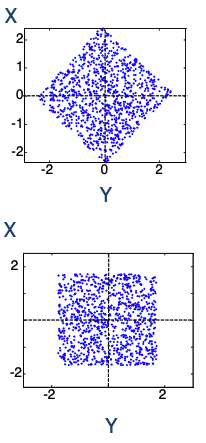
\includegraphics[width=0.18\textwidth]{images/uncorr-vs-indep.png}
          \end{center}
          \caption{Uncorrelation vs Independence}
          \label{fig:uncorr-vs-indep}
        \end{wrapfigure}
        
        The goal of ICA is to measure independence between signals and to maximize independence (tune a transformation to get independent outputs). Independence can be written as:
        \begin{align*}
            P_X(X|Y) = & \;\;\frac{P_{X,Y}(X,Y)}{P_Y(Y)} \text{\,\,(general case , conditional distribution)}\\
            \text{(given independence)}\,\,\Rightarrow &\;\;P_{X,Y}(X,Y) = P_X(X)P_Y(Y) = P_X(X|Y)P_Y(Y)
        \end{align*}
        
        Figure \ref{fig:uncorr-vs-indep} shows the difference between PCA that creates a maximum variance projection (top image) where there is no correlation but there is dependence and ICA (bottom image) which has minimum dependence directions (cannot say anything on Y knowing X).\\
        
        Whitening is preserved for any rotation while independence is conserved only for rotations of $k\frac{\pi}{2}$ with $k$ integer, up to permutation and sign.
    
    \paragraph{Difference between ICA and PCA}
        \begin{itemize}
            \item Independence is stronger than uncorrelation.
            \item If $V^\Tr$ is a whitening matrix, $UV^\Tr$ with $U$ orthogonal is a whitening matrix too. A whitening matrix is highly non-unique (up to any rotation matrix $U$)
            \item $W^\Tr$ of ICA is unique, up to a few indeterminacies.
        \end{itemize}
        
    \subsection{ICA Problem}
        We have independent (unknown) source signals 
        $$s(t) = [s_1(t), s_2(t), …, s_n(t)]^\Tr$$ 
        Measured signals 
        $$x(t) = [x_1(t), x_2(t), …, x_n(t)]^\Tr$$ 
        And a linear mixing : $x(t) = As(t)$ with $A$ unknown. We wish to determine $W^\Tr \approx A^{-1}$ such that $y = W^\Tr x = W^\Tr A s \approx s$ and use the independence hypothesis to find $W^\Tr$.
        
        \paragraph{Identifiability Theorem} ICA solves this by measuring independance between the signals $y_i(t)$ and when it is reached, it is known that $y(t) \approx s(t)$.
        
        \paragraph{Indeterminacies} ICA yields the original signals up to these indeterminacies: the order of signals as independence is symmetric and a scaling factor multiplying each signal : 
        $$x_i = \sum_{j=1}^n a_{ij}s_j = \sum_{j=1}^n \alpha a_{ij} \frac{s_j}{\alpha}$$
        The true solution is $W^\Tr = P D A^{-1}$ where D is a diagonal matrix to re-scale signals, and P is a permutation matrix (not very important in real applications).
        
        \paragraph{Solution assumptions and problem hypotheses}
        \begin{itemize}
            \item Mixtures are linear and additive
            \item Random variables are seen as signals in time
            \item Without (phase) delay
            \item Since the magnitude of $s_i$ cannot be known it is arbitrarily fixed such that $\mathbb{E}[s_i s_i^\Tr] =1$, meaning that $\mathbb{E}[s s^\Tr] = I$.
        \end{itemize}
    
    \paragraph{PCA before ICA} PCA is used as a preprocessing step to ICA. Indeed we unmix $z$, the whitened signals of $x$ rather than directly $x$. Indeed, if $z$ is white, $V^T A$ is orthogonal : 
    $$I = \mathbb{E}[zz^\Tr] = V^\Tr A \mathbb{E}[s s^\Tr] A^\Tr V = (V^\Tr A) (V^\Tr A)^\Tr$$
    And if $V^\Tr A$ is orthogonal, $W$ is orthogonal as well since we want white outputs : $$I = \mathbb{E}[yy^\Tr] = W^\Tr \mathbb{E}[zz^\Tr]W $$
    And if $W$ is orthogonal, it is symmetric and there are only $\frac{n(n-1)}{2}$ parameters to find rather than $n^2$.
    
    \paragraph{Gaussian Case} When signals are Gaussians, it is impossible to find original signals, indeed, in the Gaussian case, since density is perfectly described by mean and variance, uncorrelation and independence are identical, therefore, rotation after whitening is useless. In that case other information is needed (temporal structure, etc.). An additional assumption to ICA is then that no source is Gaussian.
    
    \noindent According to the central limit theorem, the PDF of a sum of n independent random variables tends to be Gaussian.
    
    \subsection{Non-gaussian approach}
        \paragraph{General Idea} if we consider an output of the ICA process: $y_i = c_i^\Tr s$ with $c_i = w_i^\Tr V^\Tr A$. If $c_i$ is not a solution to the ICA problem then $y_i$ is still a mixture and $c_i \approx \alpha [\pm 1/n,\pm 1/n, …, \pm 1/n]^\Tr$. This is close to the mean of several RV and by the CLT $y_i$ will be closer to a Gaussian than to a source. However, if $c_i$ is a solution to the ICA problem, $c_i = \alpha [0,…, \pm 1, …, 0]^\Tr $, which is far from the assumptions of the CLT (no sum of RV) and we will be far from Gaussianity since no source is Gaussian. The following methods measure closeness to a gaussian. 
        
        \paragraph{Method 1 : Minimum differential entropy} For this method we will use entropy:
        \begin{itemize}
            \item Discrete case: $H(x) = -\sum_{i=1}^K p_i log(p_i)$, which is minimum when $\exists i | p_i = 1, p_j = 0 \text{ for } j \neq i$ : $H(x) = 0$ and maximum when $p_i = 1/K$ : $H(x) = log(K)$.
            \item Continuous case (differential entropy) : $h(U) = -\int_{-\infty}^\infty p_U(u)log(p_U(u))du$ which is maximum when $U$ follows a Gaussian : $h(u) \leq h(u_G) = \frac{1}{2}log(2\pi e \sigma^2)$ where $\sigma^2$ is the variance of $u$. And in $n$ dimensions:
            $$h(X) \leq \frac{1}{2}log\left((2\pi e)^n det \Sigma\right)$$
            Where $\Sigma$ is the covariance matrix, $\Sigma = I$ for $h(Z)$.
        \end{itemize}
        The goal is to find $W$ such that output entropies are low, i.e. finding $w_i$ such that the pdfs of $y_i$ are far from Gaussians (with condition that $y_i$ have unit variance).
        
        \paragraph{Method 2 : Negentropy} Negentropy is defined as the difference with respect to the cross-entropy of a Gaussian with same variance : 
        $$J(X) = h(X, X_G) - h(X) \geq 0$$
        $$J(X) = \int p_X(u) log\left(\frac{p_X(u)}{p_{X_G}(u)}\right)du$$
        The goal is to find $W$ such that $J(y)$ is maximum (with condition that $y_i$ have unit variance).
        
        \noindent The difficulty of this method is that we don't know the samples's pdf's.
        
        \paragraph{Method 3 : Moments and cumulants} Rather than using PDFs for $y_i$ we use their distribution properties: moments and cumulants. And in particular the curtosis (4-th order centered moment): 
        $$\kappa_4(X) = \mathbb{E}[X^4] - 3(\mathbb{E}[X^2])^2$$
        For a Gaussian PDF, we have $\kappa_4(X_G) = 0$ and for (almost) any non-Gaussian PDF: $|\kappa_4(X)|>0$.\\
        The goal is then to find $W$ such that $\sum_{i=1}^m|\kappa_4(Y_i)|$ is maximum (with condition that $y_i$ have unit variance).\\
        
        This method is based on the Gram-Charlier Expansion (analog to Taylor expansion) which approximates a PDF around the Gaussian PDF $\varphi$ (4th order approximate) :
        $$p_X(\xi) \approx \varphi(\xi)\left(1 + \kappa_3(X)\frac{H_3(\xi)}{3!} + \kappa_4(X)\frac{H_5(\xi)}{4!}\right)$$
        Where $H(\cdot)$ are the Chebyshev-Hermite polynomials. This can be done because Kurtosis is linear if $s_i$ are independent.
    
    \subsection{Minimum dependence approach}
        \paragraph{Method 1 : Minimum Mutual Information} Mutual information is defined as: 
        $$I(X) = \int P_X(u) log\left(\frac{P_X(u)}{\prod_{i=1}^n P_{X_i}(u_i)}\right)du \geq 0$$
        Which is exactly null iff each $x_i$ is independent. It can be expressed as:
        \begin{align*}
            I(y) &= \sum_{i=1}^m h(y_i) - h(y)\\
            &= \sum_{i=1}^m h(y_i) - h(Wz)\\
            &= \sum_{i=1}^m h(y_i) - h(z) - log(|det(W)|)
        \end{align*}
        And $|det(W)| = 1$ as $W$ is orthogonal.
        The goal is to find $W$ such that $I(y)$ is minimum. But it is difficult to estimate the joint PDF of y and the computational cost is high. An alternative is to minimize the sum of output marginal entropies : $\sum_{i=1}^n h(y_i)$ where there is no need to estimate a joint PDF.
        
        \paragraph{Method 2 : Cancelling cross-cumulants} We extend the idea of PCA (diagonalization of the covariance matrix and scaling) to take into account moments of order higher than 2. It is then a diagonalization of the 4-th order tensor (4 dimensions) of cross-cumulants in order to go further than (linear) decorrelation. 
        $$cum(X_i, X_j, X_k, X_l) = \mathbb{E}[X_i X_j X_k X_l] - \mathbb{E}[X_i X_j]\mathbb{E}[X_k X_l] - \mathbb{E}[X_i X_k]\mathbb{E}[X_j X_l] - \mathbb{E}[X_i X_l]\mathbb{E}[X_j X_k]$$
        To reach independence, all cross-cumulants must be equal to 0, i.e. find a rotation matrix via the JADE algorithm (Joint Approximate Diagonalization of Eigenmatrices)
        
    \subsection{In practice}
        Independence metrics require the knowledge of the PDF which is unknown. In practice we use density estimation (difficult) or measure independence indirectly (cross-cumulants).
        
        \paragraph{PCA in ICA} pre-whitening reduces the number of elements to estimate but can lead to computational problems and errors if PCA failed. 
        
        \paragraph{Objective functions} It is also possible to minimze objective functions (non-Gaussianity and independence measures) at the risk of getting a local minima. Minimization algorithms include (natural) gradient descend, diagonalization of cross-cumulants, fixed-point iteration, etc.
        
        \paragraph{Criterions} The criterions evaluated are local criterions that can lead to local minima. The true measure of independence only leads to a global minima.
    
    \subsection{Extensions of ICA}
        The basic model is : $x_i(t) = \sum_{j=1}^N a_{ij} s_j(t)$ for $i = 1, …, N$
        \paragraph{N observed mixtures, M sources}
        \begin{itemize}
            \item $N > M$, $M$ must be estimated and during the PCA stage, there is a reduction from $N$ to $M$ signals and then source separation is applied (ICA). 
            \item $M > N$, the $N$ ``most powerful'' sources will be estimated by ICA but will be corrupted by the $M - N$ other sources. 
            \item $N >> M$, projection in signal subspace must be used.
        \end{itemize}
        
        \paragraph{Noisy observations} if the observations are noisy: 
        $$x_i(t) = \sum_{j=1}^N a_{ij}s_j(t) + n_i(t) \text{ for } i = 1, …, N$$
        $$x(t) = As(t) + n(t)$$
        Even if $W$ is estimated perfectly: 
        $$y(t) = W^\Tr x(t) = W^\Tr A s(t) + W^\Tr n(t)$$
        
        \paragraph{Other extensions} The following problems require \emph{specific algorithms}:
        \begin{itemize}
            \item \textbf{Convolutive mixtures} 
            $$x(t) = A(t) * s(t)$$
            $$x_i(t) = \sum_{j=1}^N \sum_{k=0}^{p-1} a_{ij}(k) s_j(t-k) \text{ for } i = 1, …, N$$
            \item \textbf{Post non-linear mixtures}
            $$x_i(t) =f_i\left(\sum_{j=1}^N a_{ij} s_j(t)\right) \text{ for } i = 1, …, N$$
            \item \textbf{Non-linear mixtures} 
            $$x_i(t) =f_i(s_1(t), …, s_N(t)) \text{ for } i = 1, …, N$$
            \item \textbf{Ill-conditioned mixtures} the rows of $A$ are identical ($A$ not invertible) or very similar .
        \end{itemize}

\section{Feature selection}
    \label{sec:featuresel}
    
    \subsection{Background}
        \paragraph{Motivation} Many data analysis tools suffer from high dimensionality:
            \begin{itemize}
                \item \textbf{Linear tools} PCA is based on the covariance matrix which grows in the square of the dimension and is poorly estimated on a finite number of data. Similar problems arise for Linear Discriminant Analysis (LDA), Partial Least Squares (PLS), etc.
                \item \textbf{Non-Linear tools} Tools of the form $y = f(x_1, x_2, …, x_d, \theta)$ suffer as well. As $d$ increases, so does the size of $\theta$. And as $\theta$ results from the minimzation of a non-convex functions there is a higher risk of local minima, numerical problems (flats and high slopes), convergence issues, … This affects Multilayer Perceptrons (MLP), Gaussian Mixtures (RBF), Self-Organizing maps (SOM), etc.
            \end{itemize}
        
        \paragraph{Curse of dimensionality examples}
            \begin{itemize}
                \item The number of points on a grid increases exponentially with the dimension. 
                \item \textit{Silverman, 1996} The number of Gaussian kernels necessary to approximate a Gaussian distribution grows exponentially with the dimension of the data space. To estimate parameters there is need of too much data. Histograms are used in higher dimension and are a compromise between accuracy and number of data in each bin.
                \item The volume of a sphere in high dimensions rapidly tends to 0 with the dimension of the space.
                $$V(d) = \frac{\pi^{d/2}}{\Gamma(d/2+1)} r^d$$
                \item The ratio of a sphere to a cube also rapidly tends to $0$ in high dimensions (all points are in the cube, but in the exterior of the sphere).
                \item Volume ratio of embedded spheres. In high dimensions, volume is ``concentrated'' in the outer parts of the sphere.
                \item The percentage of points following a multi-dimensional Gaussian inside a sphere of a fixed radius tends to zero.
                \item The probability to find a point at distance $r$ of the center for a multi-dimensional multi-normal distribution is higher for higher dimensions. 
                \item Euclidean norms concentrate for random vectors with i.i.d. components in $[0, 1]$ are in $[0, \sqrt{d}]$ and concentrate around their expectations in higher dimensions (they don't disciminate anymore).
                \item In the same way distances concentrate. Indeed pairwise distances seem nearly equal for all points. Relative contrast vanishes as dimension increases. If $\lim_{d\rightarrow\infty} \frac{\sqrt{Var[\|X\|_2}]}{\mathbb{E}[\|X\|_2]} = 0$ then $$ \plim_{d\rightarrow \infty}\frac{d_{max} - d_{min}}{d_{min}}=0$$
            \end{itemize}
        \paragraph{Uses} In theory it is not useful, more information means easier task and models can ignore irrelevant features (weights set to 0). However, lots of inputs means lots of parameters and large input space. This implies the curse of dimensionality and the risk of overfitting. Feature selection can be used for many reasons.
        \begin{itemize}
            \item To visualize data in lower dimensions
            \item To get insight about the causes of a problem
            \item To reduce data collection time/cost, computation time, etc.
        \end{itemize}
        
        \paragraph{Key elements} Subset relevance assessment (among $2^d - 1$ possible subsets of feature, which is the best) and Optimal subset search (how not to consider $2^d - 1$ subsets).
        
        \paragraph{Filter Approach} Filters are a model-free technique that use a relevance criterion that is not the final criterion to decide if a feature is useful or not. A variable (or set of variables) is relevant if it is statistically dependent on $y$: $P(y | x_i) \neq P(y)$ 
        
        \paragraph{Wrapper approach} Wrappers use the (non)linear model to evaluate performance of feature selection (many models to design). A variable (or set of) is relevant if the model built on it shows good performances : $\min_f (y-f(x_i))^2 \approx 0$
        
    
    \subsection{Filters}
        \subsubsection{Correlation} 
            \paragraph{Definition} Correlation between a random variable $X$ and a random variable $Y$ is 
            $$\rho_{XY} = \frac{\mathbb{E}[(X - \mathbb{E}[X]) (Y - \mathbb{E}[Y])]}{\sqrt{\mathbb{E}[(X - \mathbb{E}[X])^2] \cdot \mathbb{E}[(Y- \mathbb{E}[Y])]^2} }$$
            And is estimated as
            $$r=\frac{\sum_{j=1}^N((x_j-\bar{x})(y_j-\bar{y}))}{\sqrt{\sum_{j=1}^N((x_j-\bar{x})^2)\sum_{j=1}^N((y_j-\bar{y})^2)}}$$
            
            It measures linear dependencies, $r \in [-1, 1]$ and is null if there is no \textbf{linear} relation but low correlation does not mean the absence of relationship. High correlation does not mean causality either.
            
            \paragraph{Properties} It is linear and parametric (makes the hypothesis of a linear model), does not explain (correlation does not imply causation), is hard to define for more than two variables, and is very sensitive to outliers.
        
        \subsubsection{Mutual Information}
            \paragraph{Definition} Mutual information between a random variable $X$ and a random variable $Y$ measures how the uncertainty of $Y$ is reduced when $X$ is known (and vice versa).
            
            \paragraph{Entropy} The entropy of a random variable is a measure on its uncertainty
            \begin{align*}
                H(Y) &= -\mathbb{E}[log(P[Y])]\\
                &= - \sum_{y \in \Omega} log(P[y])P[y] \text{ for $Y$ discrete}\\
                &= - \int log(P[y])dy \text{ for $Y$ continuous}
            \end{align*}
            It can be interpreted as the average number of bits needed to describe $y$.
            
            \paragraph{Conditional Entropy} $H(Y | X)$ measures the uncertainty on $Y$ when $X$ is known
            $$H(Y | X) = H(Y, X) - H(X)$$
            If $Y$ and $X$ are independent, $H(Y | X) = H(Y)$. The uncertainty on $Y$ is the same if we know $X$ as if we don't.
            
            \paragraph{Mutual Information} The mutual information between a random variable $X$ and a random variable $Y$ is the difference between the entropy of $Y$ and the entropy of $Y$ when $X$ is known.
            $$I(Y, X) = H(Y) - H(Y|X) = H(X) - H(X |Y)$$
            
            \paragraph{Properties} $I(Y, Y) = H(Y)$ and $I(Y, X)$ is always non-negative and less than $min(H(Y), H(X))$. If $X$ and $Y$ are independent, then $I(Y, X) = 0$. It identifies non-linear relationships between variables.
            
            \paragraph{Relevance of a set of features} $X$ and $Y$ can be vectors. If $X$ is a subset of features, its relevance may still be evaluated. 
            
            \paragraph{Issues} It is very difficult to estimate $I(Y, X)$; histograms, kernels and splines suffer from the curse of dimensionality as well. k-NN estimators are more robust.
            
            \paragraph{In practice} When dealing with bivariate mutual information only, the goal is to maximize relevance $I(X_i, Y)$ while reducing redundancy $I(X_i, X_j)$. This is a multi-objective criterion that depends on the weighing between the two criteria.
            
            \paragraph{Extensions} Some extensions to mutual information exist for tri-variate mutual information (interaction measure, etc.)
            
            \paragraph{Stopping criterion} In theory, mutual information of a set of variables can only increase when adding variables. It is a bad idea to stop when MI decreases (the estimation is not valid anymore). It is better to evaluate the statistical relevance (hypothesis test) of adding a new variable. Usually a fixed maximum number of variables is set.
    \subsection{Wrappers}
        \paragraph{General idea} Building models and evaluating them on the final criterion. However, each model needs to be trained and fitted for hyper-parameters (cross-validation) and its performances must be evaluated (double cross-validation) which is computationally expensive for some models.
    
    \subsubsection{Filter-Wrapper Comparison}
        Table below shows a comparison between the filter and wrapper approach
        \begin{center}
            \begin{tabular}{|c|p{0.3\textwidth}|p{0.3\textwidth}|}
                \hline
                 & \textbf{Filters} & \textbf{Wrappers} \\\hline
                Advantages & \textbf{Fast} (only one model is built) and \textbf{intuitive} (identify statistical dependency) & Relevance criterion is \textbf{easy to estimate} and they are \textbf{model-aware} (identify optimal subset for optimal model)\\\hline
                Disadvantages & Relevance criterion is \textbf{hard to estimate} and they are \textbf{model-ignorant} (most relevant subset might not be optimal for subsequent model) & \textbf{Slow} (must build lots of models) and \textbf{not intuitive} (features for best model might not actually be most explanatory variables)\\\hline
            \end{tabular}
        \end{center}
    
    \subsection{Greedy search method}
        In theory all $2^d - 1$ subsets should be tried and evaluated but in practice, a greedy procedure is used to
        \begin{enumerate}
            \item Define an initial subset
            \item Choose a strategy to update subset
            \item Decide when to stop
        \end{enumerate}
        
        \noindent It makes the hypothesis that the best subset can be constructed iteratively.
        
        \subsubsection{Forward Search}
            \paragraph{Initial subset} An empty set is chosen.
            \paragraph{Update strategy} Either filter approach (add feature that increases the most the relevance/redundancy compromise) or wrapper approach (add features that increases the most the performances of the model)
            \paragraph{Stopping} If using a filter, a supplementary criterion is needed, if using a wrapper, stop when adding features increases the generalization error.
        
        \subsubsection{Backward search}
            \paragraph{Initial subset} An full set is chosen.
            \paragraph{Update strategy} Either filter approach (remove feature that decreases the most the relevance/redundancy compromise) or wrapper approach (remove features that decreases the most the performances of the model)
            \paragraph{Stopping} If using a filter, a supplementary criterion is needed, if using a wrapper, stop when removing features increases the generalization error.
        
        \subsubsection{Forward-Backward Search} 
            At each step, consider all additions and removals of one variable and select the best result. This makes sense with a wrapper approach but with the filter approach the mutual information cannot increase with less variables.
    
    \subsection{Genetic Algorithms}
        This method is a random exploration of the space of subsets. It is based on the following steps:
        \begin{itemize}
            \item Draw initial population (candidate subsets)
            \item Select best individuals
            \item Apply cross-overs and mutation on individuals
            \item Repeat from 2 until new population is generated
            \item Select best individuals and repeat from 1
        \end{itemize}
    
    \subsection{Embedded Methods}
        \paragraph{General Idea} Creating the model and restrict the number of features used by the model together. Optimizing the whole can only be better than separating into 2 parts.
        
        \paragraph{Example} Lasso is a linear model that does this by regularizing its weights while optimizing the model: $y = WX$ and 
        $$\min_W \frac{1}{N}\sum_{j=1}^N (y^j - Wx^j)^2 + \mu \|W\|_1$$
        Usually (Ridge Regression) the regularization term is a 2-norm. Here, the 1-norm reduces the effective number of features used by the model, both in theory and in practice.
    
    \subsection{Applications and examples}
        \paragraph{Very high dimensional data} For the infrared spectra (Tecator) the data is very high dimensional (sometimes 1000, 2000 wavelengths). Estimation of Mutual Information is very hard. Two solutions are possible : 
        \begin{itemize}
            \item Ranking the $X_i$ according to their mutual information with the output (does not take into account the relations between the $X_i$
            \item Forward selection on $I((X_i, X_j, X_k, …), Y)$ but the curse of dimensionality prevents a good estimation of the mutual information
        \end{itemize}
        A solution is to take a set of features selected by forward search (until decrease) and a set of features selected by ranking (until the union of the two reaches $N$ elements) and try the $2^N$ evaluation (either by filter or wrapper approach)
        
        \paragraph{Time series} Time series can be modeled using different sets of data:
        \begin{itemize}
            \item Sampling frequency
                \begin{align*}
                    x(t+1) &= f(x(t), x(t-1), x(t-2), x(t-3), …)\\
                    x(t+1) &= f(x(t), x(t-1), x(t-4), x(t-7), …) 
                \end{align*}
            \item Size of the regressor
                \begin{align*}
                    x(t+1) &= f(x(t), x(t-1), x(t-2), x(t-3), …)\\ 
                    x(t+1) &= f(x(t), x(t-1), x(t-2)) 
                \end{align*}
            \item Non-contiguous values
                \begin{align*}
                    x(t+1) &= f(x(t), x(t-1), x(t-2), x(t-3),x(t-4),  …)\\
                    x(t+1) &= f(x(t), x(t-1), x(t-7), x(t-8), x(t-14), …) 
                \end{align*}
        \end{itemize}
        If a time series has an intrinsic dimension of $q$ then the size of the regressor must be in $\{q, …, 2q+1\}$. Meaning that in the $2q+1$ space there exists a $q$ surface without intersecting points and it is possible to project from $2q+1$ to $q$ dimensions. \\
        
        In practice, many inputs variables are taken, $2q+1$ are selected through feature selection and if needed they are projected on $q$ new variables.

\section{Model generation}
    \label{sec:modelgen}
    \subsection{Linear regression}
        \begin{minipage}[b]{0.9\linewidth}
            \begin{itemize}
            	\item \textbf{Main notation:} $y = w^\Tr x$, with $x=(1,x_1,x_2,...,x_N)^\Tr$ and $w=(w_0,w_1,w_2,...,w_N)^\Tr$.
            	\item \textbf{Error criterion (MSE)}: $\frac{1}{P}\sum_{p=1}^P(t_p - w^\Tr x_p)^2=\frac{1}{P}\|t-w^\Tr X\|^2$
            	Where $t_p$ are the P targets to predict. \warn $X$ could be transposed!
            	\item \textbf{Down side of the MSE:}
                    \begin{itemize}
                        \item it gives a very large weight to large errors.
                        \item a single or a few outliers may influence a lot the criterion.
                    \end{itemize}
            \end{itemize}
        \end{minipage} \hfill
        \begin{minipage}[b]{0.2\linewidth}
            \centering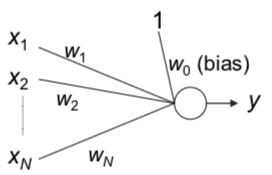
\includegraphics[width=0.9\textwidth]{images/linear-regression.png}
        \end{minipage}%\vspace{\baselineskip}
    
    \subsubsection{Pseudo-inverse $\rightarrow$ minimise the error using a gradient}
    \begin{itemize}
    	\item \textbf{Derivative of error criterion}: $\left(\diffp{E}{w}\right)^{\!\Tr} \equiv\left(\frac{\partial E}{\partial w_{1}} \frac{\partial E}{\partial w_{2}} \cdots \frac{\partial E}{\partial w_{D}}\right)$\\
    	
    	$ \frac{\partial E}{\partial \boldsymbol{w}_{j}} = \frac{\partial}{\partial w_{j}}\left(\frac{1}{P}\left({t}^{\top}-{w}^{\top} {X}\right)\left({t}-{X}^{\top} {w}\right)\right) = \frac{2}{P}(w^\Tr X-t^\Tr )X^\Tr $
    	\item \textbf{Minimum error at}: $w=(XX^\Tr )^{-1}Xt$
    	\item \textbf{Pseudo-inverse cond’s}:
            \begin{itemize}
            \item requires all input-output pairs ($x_p, t_p$)
            \item does a matrix inversion $\rightarrow$ the gradient descent doesn't need one.
            \end{itemize}
        \end{itemize}
    \subsubsection{Gradient descent}
    \begin{itemize}
    	\item \textbf{General formula}: $x(t+1) = x(t)-\alpha \diffp*{f}{x}{x(t)}$
    	\item \textbf{Gradient descent applied on error criterion}: $w(t+1) = w(t) + \frac{2\alpha}{P}X(t-X^\Tr w(t))$
    	\item \textbf{Stochastic gradient descent}: As we can write that $E=\frac{1}{P}\sum_{p=1}^PE_p$, we can optimize the $E_k$ one at a time. $w(t+1) = w(t) + \frac{2\alpha}{P}(t_k - w(t)^\Tr x_k)x_k$    %(t-x_k^\Tr w(t))x_k$
    \end{itemize}
    
    \begin{minipage}[c]{0.9\linewidth}
    \subsubsection{Classification with linear regression}
        Just use targets = ±1 if you have 2 classes. The separation will be the plane of equation $w^\Tr x=0$.
        \end{minipage}
        \begin{minipage}[c]{0.08\linewidth}
            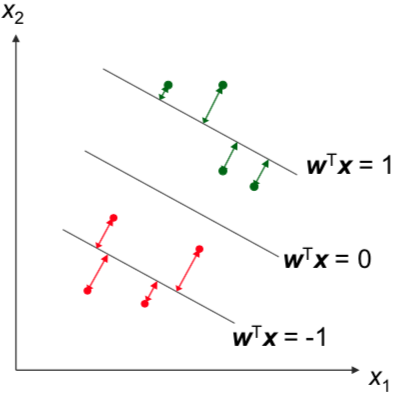
\includegraphics[width=\linewidth]{images/linear-classification.png}
        \end{minipage}
        
    % \subsubsection{Linear associative memory}
    % \begin{itemize}
    % 	\item Learning: $w=\sum_{p=1}^P t_px_p$.
    % 	\item Magic: iff $x$'s are orthogonal and normalized.
    % \end{itemize}
    
    \subsubsection{Perceptron}
    \begin{itemize}
    	\item Classification model (with output $-1$ or $1$) with $sign$ as activation function $\rightarrow t = sign(w^\Tr x)$
    	\item Object is correctly classified if $w^\Tr x_kt_k > 0$
    	\item \textbf{Ideal error criterion}: $E = \sum_{w^\Tr x_kt_k < 0} 1$ (not continuous)
    	\item \textbf{Perceptron criterion}: $E = -\sum_{w^\Tr x_kt_k < 0} w^\Tr x_kt_k$ (continuous, but gradient is only piece-wise linear). Minimising this criterion is equivalent to minimise the distance with the classifier. It doesn't minimise the count of miss-classification!
    	\item \textbf{Stochastic gradient descent on perceptron learning rule:}  $w(t+1) = w(t) + \alpha x_k t_k$
    	\item \textbf{Perceptron convergence theorem}: If a set is linearly separable, then gradient descent on the perceptron criterion will converge in a finite number of steps. Proof: verify that $\|w\|$ grows slower than $\sqrt{n}$ and that $w^\Tr_{sol}w$ is bounded below by a linear function of $n$. However, the found classifier will not always be the best.
    \end{itemize}
    \subsection{Multi-layer perceptron}
    \subsubsection{Single layer}
    Model identical to linear regression, but with nonlinear activation function.
    \begin{itemize}
    	\item \textbf{Activation function}: $\sigma(w^\Tr x)$
    	\item \textbf{Error function}: $E = \frac{1}{P}\sum_{p=1}^P(t_p - \sigma(w^\Tr x_p))^2$
    	\item \textbf{Stochastic gradient descent rule}: $w(t+1) = w(t) + \frac{2\alpha}{P}(t_k - \sigma (w(t)^\Tr x_k))x_k \diffp*{\sigma}{p}{p=w(t)^\Tr x_k}$
    	%$w(t+1) = w(t) + \frac{2\alpha}{P}(t-x_k^\Tr w(t))x_k \diffp*{\sigma}{p}{p=w(t)^\Tr x_k}$
    \end{itemize}
    
    \begin{minipage}[b]{0.75\linewidth}
    \subsubsection{Commonly used non-linear activation function}
        If we want to use the logistic function, we should use: $2 \times logistic -1$ to have it centered from $-1$ to $1$. It can be used to estimate posterior probabilities.
        
        The impact of outliers is highly reduced as those functions have an upper-bound of 1.
        \end{minipage}\hfill
        \begin{minipage}[b]{0.21\linewidth}
            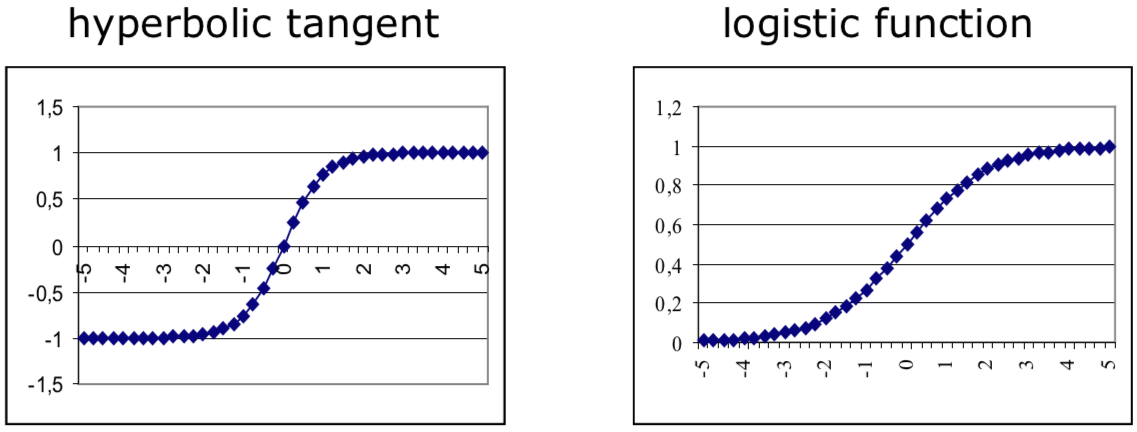
\includegraphics[width=\linewidth]{images/activation-fct.png}
        \end{minipage}
    
    \subsubsection{Multi-layer}
        \begin{itemize}
        	\item \textbf{Model}:  $y(x) = h(w^{(2)}g(w^{(1)}x))$, $h$ can be linear, but not $g$ (otherwise, \textit{this 2--layer} network can be represented by a single--layer network). The output of $g(w^{(1)}x)$ can be seen as the input of the second layer.
        	
        	The sigmoid or hyperbolic tangent are at least used for the hidden layers as non-linear activation functions.
        	
        	\item \textbf{Universal approximation property}\label{universal_approx_theorem}:  A 2-layer MLP (1 hidden layer) can approximate arbitrarily well any (functional) continuous mapping, provided the number M of hidden units is sufficiently large.\\
        	In practice, we overfit if M is too high.
        	
        	\item \textbf{Learning: Algorithm}\\
                \begin{minipage}[c]{0.75\linewidth}
        	      \begin{enumerate}
        		      \item Apply an input vector $x_k$ through the network, computing all values
        		      \item Evaluate error  on the last layer (difference with $t_k$)
        		      \item Back-propagate the error on each layer
        		      \item Compute all the derivatives of $E$
        		      \item Gradient descent step
        	      \end{enumerate}
                \end{minipage}\hfill
                \begin{minipage}[c]{0.2\linewidth}
                    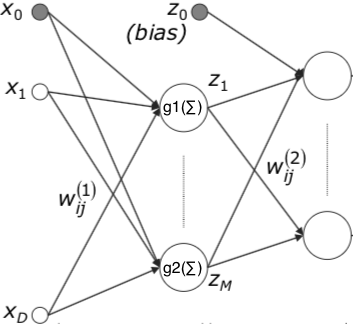
\includegraphics[width=\linewidth]{images/MLP.png}
                \end{minipage}
        \end{itemize}
    
    \subsubsection{Weight adjustment}
    
    Improvement to gradient descent (which is equivalent to the first order of Taylor):
    \begin{itemize}
    	\item \textbf{Momentum}:  $w(t+1) = w(t) - \alpha \left.\diffp{E}{w}\right|_{w(t)} {\color{blue} +  \beta(w(t)-w(t-1))}$ this blue part is new. This avoids sharp changes in gradient direction as $\beta$ is big ($\beta\approx 0.9$)
    	\item \textbf{Adaptive learning rate}: making $\alpha$ a function, increasing (resp. decreasing) by a constant when the new direction is nearly the same (resp. not the same) as previous one $$\delta w_{ij}(t-1) \, \delta w_{ij}(t) > 0 \Rightarrow \alpha_{ij} (t+1) = \alpha_{ij}(t) + \kappa$$ 
    	$$\delta w_{ij}(t-1) \, \delta w_{ij}(t) < 0 \Rightarrow \alpha_{ij} (t+1) = \alpha_{ij}(t) - \kappa$$
        
        \item \textbf{Second-order methods:}
        \begin{itemize}
            \item $E({w}(t+1))=E({w}(t))+\left(\left.\dfrac{\partial E}{\partial {w}}\right|_{{w}(t)}\right)^{T} \delta {w}+\left.\dfrac{1}{2} \delta {w}^{T} \dfrac{\partial^{2} E}{\partial {w}^{2}}\right|_{{w}(t)} \delta {w}$
            \item Stationary point: $\delta w =-\left.\left(\left.\dfrac{\partial^{2} E}{\partial w ^{2}}\right|_{ w (t)}\right)^{-1} \dfrac{\partial E}{\partial W }\right|_{ w (t)}$
            \item It ensures to make the minimum number of moves in a chosen direction. But the computation of the Hessian is heavy and it needs an inverse. We usually approximate the hessian by its diagonal terms (the first order method approximates it by a identity matrix). The inverse of a diagonal matrix is a diagonal matrix with its terms inverted.
        \end{itemize}
        
        \item \textbf{Step size adaptation: line search:} $w(t+1) = w(t) +\lambda d(t)$
        \begin{itemize}
            \item go as far as possible in the chosen direction $d(t)$
            \item if d(t) is the gradient at each time step $\left(d(t) = \left.\diffp{E}{w}\right|_{w(t)}\right)$ then $$\diffp{}{\lambda} E(w(t)+\lambda d(t))= 0\ \ \equiv\ \ \left.\diffp{E}{w}\right|_{w(t+1)} d(t) = 0$$
            So successive directions are always orthogonal. $\rightarrow$ It slows the convergence so we can use \textit{conjugate gradients} (New direction is chosen so that the component of the gradient parallel to the previous direction remains 0).
        \end{itemize}
    \end{itemize}
    
    
    \subsection{Radial-Basis Function Networks (RBFN)}
    	\paragraph{Cover's theorem} The probability of $\varphi$--separability ($\exists \textrm{ vector } w$ that linearly separates $\varphi(X)$) tends to one as more $\varphi_i$ are taken, if $\varphi_i$ are not linear and if we have more $\varphi_i$  than the number of dimensions.
    	The idea beyond this concept is that if we have an awful lot of non linear functions forming a high-dimensional space, we'll have a bigger chance that some features will be linearly separable in that space.
    	\paragraph{Interpolation problem} We search for $F:\mathbb{R}^D\rightarrow \mathbb{R}$ such that $F(x_p)=t_p, \ \forall p \in P$.
    	\paragraph{RBF Technique} $F(x) = \sum_{p=1}^P w_p \varphi\left(||x - x^p||\right)$  where $\varphi\left(||x-x^p||\right)$ are arbitrary non-linear functions (RBF). We have as many functions as data points and centers are fixed at known points $x^p$. The problem becomes an interpolation problem. In matrix form : $\phi w = t$ and $w = \phi^{-1}t$.
    	\paragraph{Michelli's Theorem} If the points $x^k$ are distinct, $\phi$ is non-singular (i.e. inversible), no matter the input space dimension. This result is valid for many RBF functions : non-localized functions like $$\varphi(x,c) = \sqrt{||x-c||^2 + I^2} \text{ with } I > 0$$ or localized functions like $$\varphi(x,c) = \frac{1}{\sqrt{||x-c||^2 + I^2}}$$ $$\varphi(x,c) = exp\left(-\frac{||x-c||^2}{2\sigma^2}\right) \text{ with } \sigma > 0$$
        \paragraph{Regularization} The criterion becomes $E(F) = \frac{1}{P}\sum_{p=1}^P(t^p - F(x^p))^2 {\color{red} + \lambda \frac{1}{P}C(w)}$. This last term smooths the output. If $C(w)$ is a problem-dependent linear differential operator, the solution is : $$F(x) = \sum_{p=1}^P w_pG(x,x_p)$$ $$w=(G+\lambda I)^{-1}t$$ $$G_{kl} = G(x^k, x^l)$$
        \begin{wrapfigure}{r}{0.4\textwidth}
          \begin{center}
            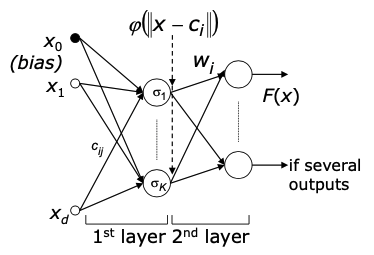
\includegraphics[width=0.33\textwidth]{images/RBFN.png}
          \end{center}
          \caption{Generalized RBFN architecture}
          \label{fig:rbfn-architecture}
          \vspace{-1cm}
        \end{wrapfigure}
    	\paragraph{Generalized RBFN} Having as many radial functions as learning patterns is computationally too intensive (matrix inversion grows in $\mathcal{O}(P^3)$), the matrix is often ill-conditioned and regularization is not easy (problem specific). We use a generalized RBFN technique with $K << P$.$$F(x) = \sum_{i=1}^K w_i\varphi(\|x-c_i\|)$$ $$\varphi(\|x-c_i\|)=\exp\left(-\frac{\|x-c_i\|^2}{2\sigma_i^2}\right)$$
    	\paragraph{Park \& Sandberg} For any function $f$, it exists a function $F$ with an unspecified $K$ that approximates $f$ as good as willed. This is the equivalent of the Universal Approximation Theorem for RBFN and gives a theoretical basis to the technique.
    	\paragraph{RBFN and kernel Regression} We wish to make a digression about (probabilistic) kernel regression: We have a non-linear regression model $t^p = f(x^p) + \varepsilon^p = y^p + \varepsilon^p$. We will estimate $f(x)$ as the average of $t$ around $x$: 
    	\begin{align*}
    	    f(x) &= \mathbb{E}[y|x]\\
    	    &= \frac{\int_{-\infty}^\infty yf_{X,Y}(x,y) dy}{f_X(x)}
    	\end{align*}
    	For this we use the Parzen-Rosenblatt density estimator (asymptotically unbiased) with K continuous, bounded, symmetric about the origin, max value at 0, with unit integral: $$\hat{f}_X(x) = \frac{1}{Ph^d}\sum_{p=1}^P K\left(\frac{x-x^p}{h}\right)$$
    	$$\hat{f}_{X,Y}(x) = \frac{1}{Ph^{d+1}}\sum_{p=1}^P K\left(\frac{x-x^p}{h}\right)K\left(\frac{y-y^p}{h}\right)$$
    	$$\Rightarrow \hat{f}(x) = \frac{\sum_{p=1}^P y^p K\left(\frac{x-x^p}{h}\right)}{K\left(\frac{x-x^p}{h}\right)}$$
    	This is equivalent to Normalized RBFN without regularization.
    	\paragraph{Learning}
    	      \begin{enumerate}
    		      \item \textbf{Centers} $c_i$: use vector quantization (FSL, competitive learning, selected at random, Kohonen maps, …) to find the centers ($c_i$ are centroids). We usually want to place centers where we have a lot of data. This phase only uses the $x^k$ information, not the $t^k$ (it is unsupervised).
    		      \item \textbf{Widths} $\sigma_i$: choose them according to the standard deviation around the centroids (local clusters). Here also only using the $x^k$ information.
    		      \item \textbf{Weigths} $w_i$: with $c_i$ and $\sigma_i$, finding $w_i$ becomes linear (as $w_i$ multiply a function that doesn't depend on $w_i$). Simply use pseudo-inverse or SVD (more used in practice).
    	      \end{enumerate}
    	\paragraph{Standard deviation of the widths}
    	      \begin{itemize}
    		      \item $\sigma = \frac{d_{max}}{\sqrt{2K}}$ where $d_{max}$ is the max distance between centroids
    		      \item $\sigma_i = \frac{1}{q}\sqrt{\sum_{j=1}^{q}\|c_i-c_j\|^2}$ where index j scans the $q$ nearest centroids
    		      \item $\sigma_i = r \min_j(\|c_i-c_j\|)$ where $r$ is an overlap constant
    	      \end{itemize}
    	      
    	\paragraph{Improvements}
            \begin{itemize}
                \item Optional computation step: gradient descent on all parameters and not only on the weigths (some improvement but problems of learning speed, local minima, risk of non-local basis functions, …). We can also choose the widths by increasing them. The first minimum found should be chosen as it is usually less sensitive to variability and preserves the locality of clusters.
                \item Add constant and linear terms to $F(x)$ (useful because very difficult to approximate a constant with Kernels)
                $$F(x) = \sum_{i=1}^K w_i exp\left(-\frac{\|x-c_i\|^2}{2\sigma_i^2}\right) + \sum_{i=1}^D w_i' x_i + w'_0$$
                \item Normalize the $\phi_i$ to make them bounded to $[0,1]$ (can be interpreted as probability values, useful for classification)
                $$F(x) = \sum_{i=1}^K w_i \frac{exp\left(-\frac{\|x-c_i\|^2}{2\sigma_i^2}\right)}{\sum_{j=1}^Kexp\left(-\frac{\|x-c_j\|^2}{2\sigma_j^2}\right)}$$
            \end{itemize}
        \paragraph{Comparison with MLP}
            \begin{center}
                \vspace{-0.5cm}
                \begin{tabular}{l|l}
                    RBFN & MLP \\\hline
                    Single hidden layer & Single or multiple hidden layers\\
                    Non-linear hidden layer, linear output layer & Non-linear hidden layer, linear or non-linear output layer\\
                    Argument of hidden units: Euclidean norm & Argument of hidden units: Scalar product\\
                    Universal Approximation Property & Universal Approximation Property \\
                    Local Approximators & Global Approximators\\
                    Splitted Learning & Global Learning\\
                \end{tabular}
            \end{center}
    \subsection{Vector Quantization}
    \subsubsection{Background}
        \paragraph{Definition} Quantization is the process of mapping input values from a large set (often continuous) to output values in a (countable) smaller set. Rounding is a typical example.
        \paragraph{Uses} Very much used in digital signal processing as representing a signal in digital format entails rounding. It is also the core of essentially all \textbf{lossy} compression algorithms.
    	\paragraph{Goal} find $Q$ vectors (\textbf{centroids}) ($Q<P$), simplifying the database, while minimizing the loss of information.
    	\paragraph{Voronoi zone} (around a centroid): Subset of the space that lies closer to this centroid than to any other.
    	\paragraph{Vector quantizer} A codebook (set of centroids) $Y = \{y_i | 1 \leq j \leq M\}$ (with M the number of features) and a quantization function $q$:
    	$$q: x \xrightarrow{} q(x) = y_j$$
    	Usually $q$ is defined by the nearest neighbor rule according to some distance measure: 
    	$$q(x) = \text{arg}\min_{y_j} d(x, y_j)$$
    	\paragraph{Quantization error} The difference between an input value and its quantized value. For a finite dataset, the expectation of this error can be replaced with the average:
    	$$\mathbb{E}_X[d^2(x, y_j)] \approx \frac{1}{N}\sum_{i=1}^N d^2(x_i, y_j)$$
    	
    	\paragraph{Usual distances} These are the distances commonly used for vector quantization
        	\begin{itemize}
        	    \item \textbf{Minkowski’s $L_P$ norm} $d_p(x_i,y_j) = \left(\sum_{k=1}^D (x_{i,k} - y_{j,k})^p\right)^{1/p}$
        	\item \textbf{Euclidian distance} $d_2$, Least Squared Error. Usually used for mathematical convenience.
        	\item \textbf{Weighted distances} $d_W(x_i,y_i) = \sqrt{(x_i-y_i)^\Tr W(x_i-y_i)}$.
        	      \begin{itemize}
        		      \item \textbf{Mahalanobis distance} $W=\Gamma^{-1}$ with $\Gamma = \mathbb{E}[(x-\mathbb{E}[x])(x-\mathbb{E}[x])^\Tr]$ the covariance matrix.
        		      \item  \textbf{$W$ symmetrical} $d_W(x_i,y_j) = d_2(Px_i,Py_j)$ with $W=P^\Tr P$
        		      \item If $W = I$, we have Euclidean distance.
        	      \end{itemize}
        	 \item Other distances can be designed for application-specific purposes.
    	\end{itemize}

    \subsubsection{Lloyd's principle}
    
    	\paragraph{Lloyd's Principle} VQ is a two stage process: $x_i \rightarrow \text{encoder } \alpha \rightarrow j \rightarrow \text{decoder } \beta \rightarrow y_j$.
    	
    	\begin{itemize}
    	    \item \textbf{$\alpha$ known} best $\beta$ given by $\beta(j) = \argmin_{y_j}(E(d(x_i,y_j)|\alpha(x^i)=j))$ This is the rule of the center of mass $\rightarrow$ the index is fixed so it minimises the distance with the prototype $\rightarrow y_j$ is moved to the center of mass = mean of data points if the distance is euclidian.
    	    \item \textbf{$\beta$ known} best $\alpha$ given by $\alpha(x_i) =  \argmin_j(d(x_i,y_j)) \text{ where } y_j =\beta(j)$ This is the rule of the nearest neighbour $\rightarrow$ take the closest data point and give its codebook index to $\alpha$.
    	\end{itemize}
    	\paragraph{Lloyd's algorithm} These are the steps to Lloyd's algorithm to find a suitable quantizer.
    	      \begin{enumerate}
    		      \item Choose initial centroids
    		      \item Encode all points $x_i$ (nearest-neighbor) and evaluate current error:
    		      
    		      $E_{ VQ }( Y ; X )=\frac{1}{N} \sum_{i=1}^{N}\left\| x _{i}- y _{j\left( x _{i}\right)}\right\|^{2},$ with $j\left( x _{i}\right)=\arg \min _{j}\left\| x _{i}- y _{j}\right\|^{2}$
    		      \item If error small enough, stop
    		      \item Replace all centroids $y_j$ with the center-of-mass of the values associated to it (decoding)
    		      \item Go back to step 2
    	      \end{enumerate}
        \paragraph{Properties of the algorithm}
    	      \begin{itemize}
    		      \item \textbf{Hypothesis}: Probability of finding a point on the border of a voronoi zone is $0$
    		      \item \textbf{Limitation}: Local minimum of the error
    		      \item \textbf{Properties}: The mean square error decreases at each iteration. The risk of getting trapped in local minima is high. And the final quantizer depends on the initial one
    	      \end{itemize}
    	\paragraph{Different initialisations of Lloyd's algorithm}
    	      \begin{itemize}
    		      \item At random in the input space (no data taken into account)
    		      \item First $Q$ points of $X$
    		      \item Randomly chosen points in $X$
    		      \item Product codes: product of scalar quantizers
    		      \item Growing initial set (choose randomly in $X$, but keep only if distance to the already chosen centroids is higher than a threshold)
    		      \item Pairwise nearest neighbor (begin with all $X$, and at each step merge the two closest centroids, creating a new point at their center of mass). Variant: merge the two centroids giving the lowest increase of error. No threshold is needed for this method.
    		      \item Splitting: A random centroid $y_1$ is chosen with a second $y_2 = y_1 + \varepsilon$, apply Lloyd's algorithm, create two new centroids by perturbing the existing ones, etc. Repeat until we have $Q$ centroids.
    	      \end{itemize}
    \subsubsection{Competitive learning}
        \paragraph{Update of the centroids} For each $x_i$, change the position of the nearest centroid: $$y_k(t+1)=y_k(t)+\alpha(x_i-y_k)$$
        The error is $$E = \int\|x-y_{j(x)}\|^2 \, p(x) \dif x$$
        with p the pdf of the distribution of x. This in discrete form is the MSE.
        \paragraph{Robbins-Monro conditions on $\alpha$} $\sum_{t=0}^\infty \alpha(t) = \infty$ and $\sum_{t=0}^\infty \alpha(t)^2 < \infty$
        \paragraph{Advantages} Simplicity, adaptive algorithm (useful with streaming data), Ability to escape local minima $\rightarrow$ no guarantee though.
        \paragraph{Disadvantages} Local minima, possible to ``lose'' centroids (if the centroid is further from all data points than all other centroids)
        
    \subsubsection{Frequency-sensitive learning}
        Based on Competitive learning. To avoid to ``lose'' centroids, this method penalize those who are often selected and encourage selection of other ones.
        
        Multiplies the distances by a function $u$ that is incremented each time this centroid is selected when selecting winner.
    
    % Pas vu en 2020
    \subsubsection{Learning Vector Quantization}
    \paragraph{LVQ1}
    \begin{itemize}
    	\item With classes
    	\item Same algo as competitive learning if centroid and $x_i$ are in the same class: $y_k(t+1)=y_k(t)+\alpha(x_i-y_k)$
    	\item But increase distance of centroids of different classes than $x_i$: $y_k(t+1)=y_k(t)-\alpha(x_i-y_k)$
    \end{itemize}
    \paragraph{LVQ2}
    \begin{itemize}
    	\item Try to reaches Bayes (optimal) boundary
    	\item Selection of two winners
    	\item Move the two winners if
    	      \begin{enumerate}
    		      \item One winner ($y_{a}$) is in the same class as $x_i$ AND
    		      \item The other one($y_{b}$) is not AND
    		      \item $x_i$ is in between the two centroids, in a window of fixed size
    	      \end{enumerate}
    	\item Move: $y_a(t+1)=y_a(t)+\alpha(x_i-y_a(t))$ and $y_b(t+1)=y_b(t)+\alpha(x_i-y_b(t))$
    \end{itemize}
    \paragraph{Improvements}
    \begin{itemize}
    	\item \textbf{Forgetting factor}: progressively ignore data from boundary
    	\item \textbf{Dynamic Vector Quantization}: Add centroids if needed ($x_i$ of class 1 is the nearest point to centroid of class 2 or distance between point and centroid too wide)
    \end{itemize}
    \subsubsection{Winner-take-all/Winner-take-most}
        When two centroids are close in distance to a data point it is hard to decide between them. We chose to adapt the winner and other centroids to some extent. 
    
        \paragraph{Soft Competition Scheme (SCS)}
            The adaptation rule is : 
            $$y_j(t+1) = y_j(t) + \alpha(t)G(i,j)(x_i - y_j(t))$$
            for all j and with $G(i,j) = \frac{exp\left(-\|x_i - y_j(t)\|^2/T\right)}{\sum_{k=1}^Q exp\left(-\|x_i - y_j(t)\|^2/T\right)}$ with decreasing temperature $T$ over time.
        
        \paragraph{Stochastic Relaxation Scheme (SRS)}
            Adaptation rule is:
            $$y_j(t+1) = y_j(t) + \alpha(t)G(i,j)(x_i - y_j(t))$$
            for all j and with 
            \begin{equation*}
                G(i,j) = \begin{cases}
                            1 \text{ with probability } p\\
                            0 \text{ with probability } 1-p\\
                         \end{cases}
            \end{equation*}
            and $p = \frac{exp\left(-\|x_i - y_j(t)\|^2/T\right)}{\sum_{k=1}^Q exp\left(-\|x_i - y_j(t)\|^2/T\right)}$ with decreasing temperature $T$ over time.
    
        \paragraph{Neural Gas}
            Centroids are ranked according to their distance with $x_i$: $h(j, x_i) = c$ if $y_i(t)$ is the c-st nearest centroid from $x_i$.
            The adaptation rule becomes: 
            $$y_j(t+1) = y_j(t) + \alpha(t)exp\left(-\frac{h(j, x_i)}{\lambda(t)}\right)(x_i - y_j(t))$$ where $\lambda(t)$ is an arbitrary regulator.
            This resumes to competitive learning when $\lambda(t) = 0$. We can have a partial sorting possible or extend with Frequency sensitive learning.
            
            \noindent This method is a stochastic descent on :
            $$E_{NG}(Y, X) = \int \frac{\sum_{j=1}^Q exp(-h(j,x)/\lambda(t))\|x-y_j\|^2}{2\sum_{j=1}^Q exp(-h(j, x)/\lambda(t))}dx$$
    
    \subsection{Self-Organizing Maps}
    
    	\noindent VQ with a supplementary grid space, defining a topology. 
    	\paragraph{Topology conservation} if centroids lie closely in the grid space, they are more likely to lie closely in data space (and vice-versa).
    	\paragraph{Adaptation of weights} Take the winner $k=\argmax_i(w_i^\Tr x)$ and update the weights: $$w_j(t+1)= w_j(t) + \alpha(t)(x-w_j(t))\,V(k,j)$$
    	
    	\noindent $\alpha(t)$ and $r(t)$ decrease over time.
    	
    	\noindent $\alpha$ must follow Robbins-Monro conditions.
	
    	$\alpha(t) = \dfrac{1}{at+b}$ is often used. $\alpha(t) = -at +b$ is too slow; $\alpha(t) = \exp{-at+b}$ is too fast.
    	\paragraph{Hard neighbourhood} only neighbours \emph{in the grid space} are updated
    	$$V(k,j)=\left\{ \begin{array}{l l}
    			      1 & \text{if } d(k,j)<r(t) \\
    			      0 & \text{otherwise}
    		      \end{array}
    		      \right.$$
    	\paragraph{Soft neighbourhood}
    	all centroids' positions in the data space are updated, but their movement decreases with the distance (in the grid space) to the closest centroid of the data point $V(k,j)=\exp\left(-\frac{d^2(k,j)}{2r^2(t)}\right)$, and increases with the distance (in the data space) to the data point.
    	
    	\noindent The soft neighbourhood usually result in a smoother grid than with the hard one.
    	\paragraph{Use of euclidean distance} If we have normalized weights ($\|w_j\|=1$) and a monotonic activation function f, then maximizing the scalar product $\equiv$ minimizing the euclidean distance ($\arg \max _{j} f\left( w _{j}^{ T }(t) x _{i}\right)=\arg \min _{j}\left\| w _{j}(t)- x _{i}\right\|^{2}$). Indeed,
    	\begin{align*}
    	    \left\| w _{j}(t)- x _{i}\right\|^{2} & = \left\| w _{j}(t)\right\|^{2}+\left\| x _{i}\right\|^{2}-2 w _{j}^{ T }(t) x _{i} \\
    	    & = 1 +\left\| x _{i}\right\|^{2}-2 w _{j}^{ T }(t) x _{i}
    	\end{align*}
    	Advantages of using $d(w_i,x)$: no need for normalization, closer to regular, and distance-based vector quantization.
    	
    	\noindent Other distances may be used
    	
    	\begin{wrapfigure}[14]{r}{0.35\textwidth}
            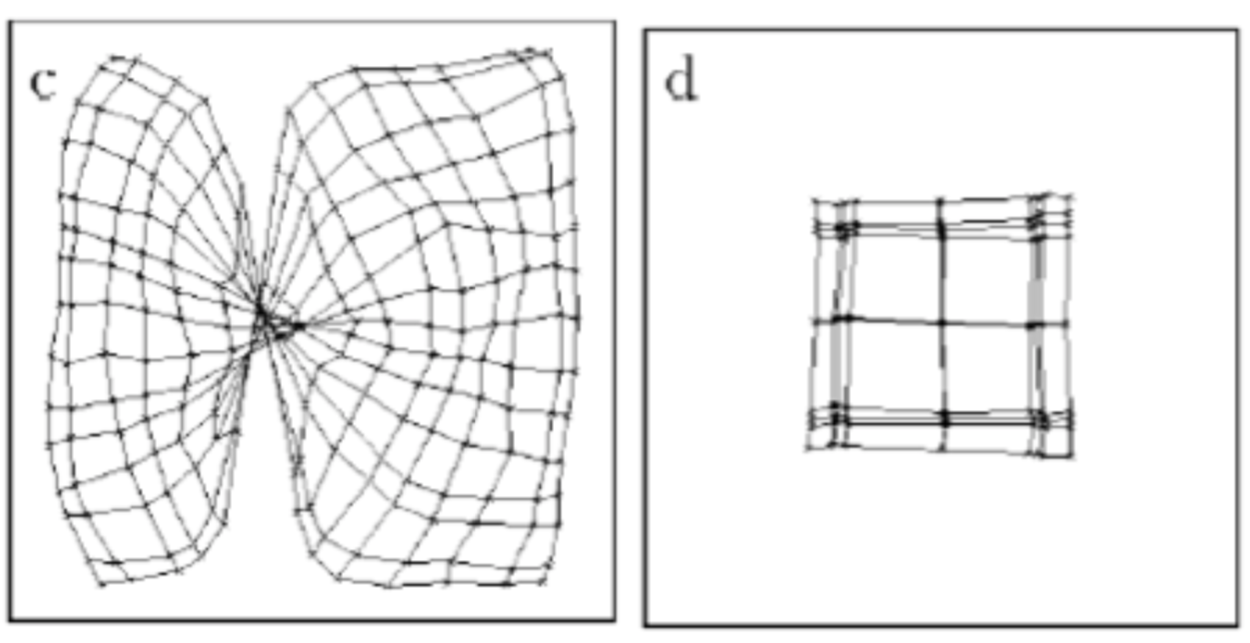
\includegraphics[width=0.33\textwidth]{images/vq-effects.png}
            \caption{Butterfly and Pinch effect}
            \vspace{\baselineskip}
            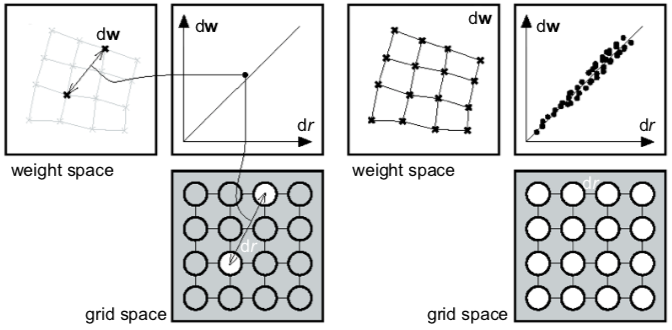
\includegraphics[width=0.33\textwidth]{images/VQ-eval.png}
            \caption{VQ quality of organization}
            \label{fig:VQ-quality}
    	\end{wrapfigure}
        
    	\paragraph{Butterfly effect} If $r(t)$ decreases too rapidly with respect to $\alpha(t)$
    	\paragraph{Pinch effect} If $r(t)$ decreases too slowly with respect to $\alpha(t)$

    	\paragraph{Choice of grid} The shape and size of grid might be inappropriate for the data. For example having two different distributions but only one grid will give surprising results.
    
    
    \subsubsection{Measures of quality}
    	\paragraph{Quality of VQ} same as VQ techniques (MSE, Ratio intra-class variance vs. inter-class variance,...)
    	\paragraph{Quality of Organization}
    	If $dw$ is the distance of centroids in weight space and $dr$ is the distance between centroids in grid space.
    	
    	\noindent Then $dw-dr$ points should be near a straight line after convergence (see figure \ref{fig:VQ-quality}). If it's not the case, one problem could be that the dimension of the grid space is too small compared to the data space (2 points in a 2D data space could be close but could be far in a 1D grid space as this space will appear to ``zig-zag'' along the data points).
    
    \subsection{Support Vector Machines (SVM)}
    A support Vector Machine is a method that generates a hyperplane (like the perceptron) that separates classes.
    
    \subsubsection{Linear}
    \paragraph{Hard-Margin} The idea is to select the hyperplane that maximizes the margin to that hyperplane. The width of that margin is : $\frac{2|k|}{\|w\|}$ with 
    \begin{equation*}
        k = \begin{cases}
            w^\Tr x + b \text{ if } x \in C^1\\
            -w^\Tr x - b \text{ if } x \in C^2
        \end{cases}
    \end{equation*} 
    The problem is then :
    \begin{align*}
        \max_{w, b} &\frac{2|k|}{\|w\|}\\
        s.t \;\;& w^\Tr x + b \geq k \;\; \forall x \in C^1\\
        & w^\Tr x + b \leq -k \;\; \forall x \in C^2
    \end{align*}
    Without loss of generality, data can be scaled such that $k = 1$. Making the problem:
    \begin{align*}
        \max_{w, b} &\frac{2}{\|w\|}\\
        s.t \;\;& w^\Tr x + b \geq 1 \;\; \forall x \in C^1\\
        & w^\Tr x + b \leq -1 \;\; \forall x \in C^2
    \end{align*}
    Defining $y^i = \begin{cases} 
        1 \text{ if } x^i \in C^1\\
        -1 \text{ if } x^i \in C^2
    \end{cases}$ constraints become : $y^i(w^\Tr x^i + b) \geq 1$ $\forall x^i$, and the problem (objective reformulated to be convex)
    \begin{align*}
        \max_{w, b} &\frac{2}{\|w\|} \text{ or } \min_{w, b} \|w\|^2\\
        s.t \;\;& y^i(w^\Tr x^i + b) \geq 1 \;\; \forall x^i
    \end{align*}
    Since the problem is convex, there is a unique global minimum value, and a unique minimizer ($w^*, b^*$ that minimizes the objective). The problem is infeasible if not linearly separable but otherwise can be solved with quadratic programming (very efficient). 
    
    \paragraph{Soft-Margin} To handle non-linearly separable datasets, we introduce slack variables $\xi^i$ that allow some points to fall within margin but who are penalized. Constraints become: 
    $$y^i(w^\Tr x^i + b) \geq 1 - \xi^i \;\; \forall x^i$$
    $$\xi^i \geq 0$$
    And the objective becomes : 
    $$\min_{w, b} \|w\|^2 + C\sum_i \xi^i$$
    Where $C$ is a parameter that trades-off margin width and misclassifications. This algorithm tries to maintain the slacks to 0 while maximizing the margin. The algorithm does not minimize the number of misclassifications (NP-complete problem) but the sum of distances to the margin hyperplane. As $C \rightarrow \infty$ the solution of the Soft-Margin tends to the solution of the Hard-Margin.
    
    \paragraph{Soft-Hard margin comparison} Soft Margins always have a solution, are more robust to outliers, have smoother surfaces in the non-linear case but the Hard-Margin does not require any parameter (Soft-Margin requires a value for $C$)

    \subsubsection{Non-linear with Kernel trick}
    To introduce non-linearities SVM uses a function $\Phi(x)$ to map to a different space:
     \begin{align*}
        \min_{w, b} &\|w\|^2 + C\sum_i \xi^i\\
        s.t \;\;& y^i(w^\Tr \Phi(x^i) + b) \geq 1 - \xi^i \;\; \forall x^i\\
        & \xi^i \geq 0
    \end{align*}
    Data then appear as $\Phi(x)$ and weights $w$ are now in the new space. Such a mapping is expensive if $\Phi(x)$ is very high dimensional. 
    
    \paragraph{The (Wolfe) Dual of the problem} The problem can be reformulated as:
    \begin{align*}
        \min_{\alpha^i} & \frac{1}{2} \sum_{i,j} \alpha^i \alpha^j y^i y^j \left(\Phi(x^j)^\Tr \Phi(x^i)\right) - \sum_i \alpha^i\\
        s.t \;\;& 0 \leq \alpha^i \leq C \;\; \forall x^i\\
        & \sum_i \alpha^i y^i =  0
    \end{align*}
    Instead of N inequality constraints, N positivity constraints, N slack variables $\xi$ and D+1 parameters ($w$, $b$), we have one equality constraint, N positivity constraints, N number of $\alpha$ variables (Lagrange multipliers) and a more complicated objective. Data now only appears as : $\Phi(x^i)^\Tr \Phi(x^j)$
    
    \paragraph{Kernel Trick} Rather than map the data in the new space and take the inner product of each pair of vectors, we can find a function such that : $K(x^i, x^j) = \Phi(x^i)^\Tr \Phi(x^j)$ and we can avoid explicitly mapping the data in the high-dimensional space (for training).\\
    
    \noindent For new instances, we can classify with:
    $$sign(w^\Tr \Phi(x) + b) = sign(\sum_i \alpha^i y^i K(x^i, x) + b)$$
    And $b$ can be extracted with (for any $j$ with $\alpha^j \neq 0$) :
    $$\alpha^j \left(y^j\sum_i \alpha^i y^i K(x^i, x^j) + b - 1) = 0 \right)$$
    
    \subsubsection{Kernels}
    \paragraph{Polynomial kernel of degree $p$} $$K(x,z)=(x^\Tr z+1)^p$$
    For $p=2$ and $D=1000$, the explicit mapping means to calculate around $D^3 = 10^6$ features and take the inner product of two $D^3$-dimensional vectors. Using kernel, it only is the inner product of two $D$-dimensional vectors and raise it to power $p=2$.
    
    \paragraph{The Gaussian kernel}$$K(x,z) = exp\left(-\frac{\|x-z\|}{2\sigma^2}\right)$$
    Which is widely used and requires a hyper-parameter ($\sigma$). In theory it maps instances to an infinite-dimensional space (difficult to explicitly write $\Phi(x)$). In practice, the dimension of feature space is the number of instances. By Cover's Theorem, the probability of linear separability in that (very high-dimensional) space is very high.
    
    \paragraph{Kernel Properties}
    \begin{itemize}
        \item Kernels must be symmetric
        \item The Gram Matrix $G^{ij} = K(x^i, x^j)$ computes the kernel for each pair of training instances.
        \item If $K_1(x,z)$ and $K_2(x,z)$ are kernels, and $p(\cdot)$ is a polynomial, then : 
        \begin{itemize}
            \item $aK_1(x,z) + bK_2(x,z)$
            \item $K_1(x,z)K_2(x,z)$
            \item $p(K_1(x, z))$
            \item $exp(K_1(x, z))$
            \item etc. 
        \end{itemize}
        are kernels too.
    \end{itemize}
    
    \paragraph{Mercer condition} There is a feature space $\Phi(x)$ when the kernel is such that $G$ is always Positive Semi Definite.
    
    \paragraph{Other Kernel methods} Multi-class SVMs, Regression SVMs, Clustering SVMs, etc. Kernels that are suitable when instances $x$ are not standard vectors but strings, infinite-dimensional objects, time series, etc. They are useful since there is no need for the instances but only the kernel distance $K(x^i, x^j)$ is sufficient.
    
    \noindent Basically any data analysis method that can be expressed as an inner product $x^\Tr z$ can use a kernel : 
    \begin{itemize}
        \item Principal Component Analysis
        \item Partial Least Squares
        \item Self-Organizing Maps
        \item etc.
    \end{itemize}

    \paragraph{Multi-class SVM} Multiple methods are possible
    \begin{itemize}
        \item \textbf{One-vs-all} Training a classifier for each class against all others and select the most confident classification (highest margin)
        \item \textbf{One-vs-one} Training $n(n-1)/2$ classifiers, each classifying a pair of classes. 
        \item \textbf{Truly Multi-class SVM} Generalization of the optimization problem to handle multiple categories.
    \end{itemize}
    
    \paragraph{SVM Variable Selection} Train a linear SVM, remove variables with lowest weights (those impacting the least the classification) with a threshold or a proportion of number of variables, retrain the SVM and repeat until the right number of variables. Possible to formulate the minimization problem of SVM with variable reduction or to extend to non-linear SVM. This is a very efficient variable selection method. 
    
    \subsubsection{Comparison with MLP}
    \begin{tabular}{l|l|l}
    	                   & MLP                            & SVM                         \\
    	\hline
    	Mapping to         & Moderate dimensional space     & Very high dimensional space \\
    	Unique minimum?    & No                             & Yes                         \\
    	Training           & Expensive                      & Efficient                   \\
    	Classification     & Efficient                      & Efficient                   \\
    	(Hyper-)parameters & Number of hidden layers \& units & kernel, kernel hyperparam, regularization cst $C$      \\
    	Robust             & Moderately                     & Yes
    \end{tabular}
    
    \subsubsection{SVM Generalization}
    No risk of overfitting because of the high-dimensional space as the model is very constrained in feature-space (because of strong bias) and the number of parameters is limited by the number of instances (solution has to be a linear combination of the training instances). Theory (Vapnik, …) gives bounds on the error of SVM (Structural Risk Minimzation) but these bounds are too loose to be of practical use except in the choice of parameters (kernel and hyperparameters)
    


\section{Model Selection}
    
    For the feature selection and model generation,
    we often need to choose a few parameters,
    e.g. the number of features, the number of neurons, ...
    
    This parameter often changes the \emph{complexity} of the model.
    As can be seen in \figuref{biasvariancecompromise}, increasing the model complexity
    obviously enables the model to decrease the error on the learning set.
    However, allowing the model to fit too much the data will allow it to start fitting the noise!
    This decreases its ability to generalize.
    In \figuref{biasvariancecompromise}, we see that the error on the validation set increases for a highly complex model.
    This phenomenon is called overfitting.
    
    If our model is not complex enough, it might miss relevant relations between features and the output,
    this is called underfitting.
    The goal of model selection is to find the compromise between underfitting and overfitting.
    
    \paragraph{Remark}
    Increasing the size of the learning set decreases the risk of overfitting.
    
    \begin{myfig}{biasvariancecompromise}{Model structure selection is a compromise between bias and variance}
    	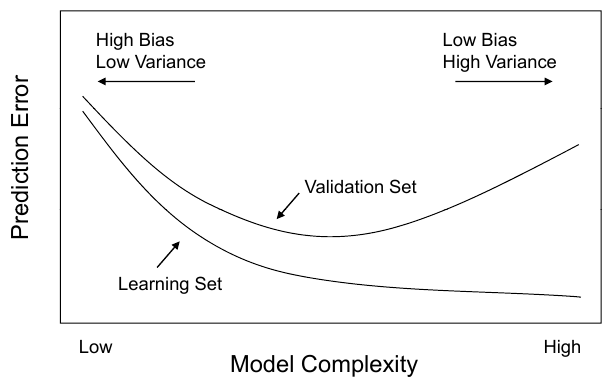
\includegraphics[width=0.6\textwidth]{images/biasvariancecompromise.png}
    \end{myfig}
    
    Different approaches exist for finding this compromise.
    For each of them, the set used for learning is reduced
    so we have even less data to find the value of the parameters of our model.
    This is the price to pay to avoid overfitting.
    
    
    \subsection*{Model selection problem}
    How to find the best model between several different ones ?
    
    Ideally, the generalization error $E_{gen}(\theta)$ of a model $g$ with hyper-parameters $\theta$ and $N$ samples can be computed as such :
    \begin{align*}
        E_{gen}(\theta) &= \int_{x} (g(x,\theta) - y(x))^2 dx \\
        &= \lim_{N\to\infty} \frac{1}{N} \sum_{i=1}^{N} (g(x_i, \theta) - y_i)^2
    \end{align*}
    But since we do not have $N\to\infty$, we have to estimate $\hat{E}_{gen} = \frac{1}{N} \sum_{i=1}^{N} (g(x_i, \theta) - y_i)^2$, with finite (sometimes small) N.
    
    \subsubsection{Regularization}
    One solution to avoid overfitting is to include a cost for high values of $w$, the weights of the model.
    That, we minimize
    \[ E(w) + \lambda\|w\|^2. \]
    This is called regularization.
    
    \subsubsection{Akaike Information Criterion (AIC)}
    We denote by $\dim(\theta)$ the dimension of $\theta$ (i.e. the number of parameters).
    For instance, if $\theta = w \in \R^n$, then $\dim(\theta) = n$.
    
    In 1973, Akaike proposed to approximate $H(W)$ with $\frac{2}{N} \dim(\theta)$ which gives the following generalization error (uses same data for training and performance evaluation, hence overfitting not detected, and estimation of generalization error is penalized with a term that depends on model complexity):
    $$\hat{E}_{gen, AIC}(\theta) = \hat{E}_{gen}(\theta) + \frac{2}{N}\dim(\theta)$$
    
    \subsubsection{Bayesian Information Criterion (BIC)/Minimum Description Length (MDL)}
    In 1978, Rissanen proposed to approximate $H(W)$ with $\frac{\ln(N)}{N} \dim(\theta)$ which gives the following generalization error:
    $$\hat{E}_{gen, BIC}(\theta) = \hat{E}_{gen}(\theta) + \frac{\ln(N)}{N}\dim(\theta) $$
    
    \paragraph{Note} Both criterion are good if the model is linear and $N$ is very large which is rarely the case.
    
    \subsection{Validation}
    \paragraph{Validation} The data set is split in a learning set of size $N_1$ and a validation set (VS) of size $N_2$. Generalization is then estimated as:
    $$\hat{E}_{gen}(\theta) = \frac{1}{N_2} \sum_{x_i \in VS} (g(x_i, \theta) - y_i)^2$$
    
    \paragraph{Cross-Validation} Make $K$ \textbf{random} repetitions of the validation with different learning sets and validation sets (always of sizes $N_1$ and $N_2$ respectively). Generalization error is estimated as:
    $$\hat{E}_{gen} (\theta) = \frac{1}{K}\sum_{k=1}^K \frac{1}{N_2} \sum_{x_i \in VS_k} (g(x_i, \theta) - y_i)^2$$
    
    \paragraph{K-fold Cross-Validation} This method is a cross-validation that ensures each data is used once and only once for each validation. The data is split in $K$ different sets and each set of size $N/K$ is used as validation against training on all other sets. This is done $K$ times. Generalization error is estimated as:
    $$\hat{E}_{gen} (\theta) = \frac{1}{K}\sum_{k=1}^K
    \frac{1}{N/K} \sum_{x_i \in VS_k} (g(x_i, \theta) - y_i)^2$$
    
    \paragraph{Leave-one-out} This method is identical to K-fold Cross-Validation with $K=N$. The validation set is then of size $1$ every time. Generalization error estimation becomes:
    $$\hat{E}_{gen} (\theta) = \frac{1}{N}\sum_{k=1}^N \sum_{x_i \in VS_k} (g(x_i, \theta) - y_i)^2$$

    \subsection{Bootstrap}
        \paragraph{General principle} The goal is to test the model on all possible data (world), but must do it on data available (sample). Problem is, using the sample for learning and evaluation leads to an optimism in the evaluation (overfitting not detected). The idea is to create a new world and sample. 
    	\paragraph{Plug-in principle} For a well-chosen new world and new sample, the difference between them will be approximately equal to the optimism. This is equivalent to using the empirical distribution of the parameter in a sample instead of the true distribution.\vspace{\baselineskip}
    	
    	Here the well-chosen new world will be the sample (all available data) and the new sample will be drawn (with replacement) from the sample. They will have the same size.
    	
    	\paragraph{Notation} $E_{A,B}$ is the error of a model learned on $A$ and tested on $B$. Meaning 
    	$$E_{gen} = E_{S,W}$$
    	With $W$ the world, $S$ the sample, $W^*$ the new world, $S^*$ the new sample.
    	
    	\newpar The optimism is:
    	$$O = E_{S, W} - E_{S,S}$$
    	The difference is:
    	$$E_{S^*, W^*} - E_{S^*, S^*} = E_{S^*, S} - E_{S^*, S^*}$$
    	
    	\noindent And Generalization error is estimated with:
    	\begin{align*}
    	    \hat{E}_{gen} &= E_{S,W} + E_{S,S} - E_{S, S}\\
    	    &= E_{S,S} + (E_{S,W} - E_{S,S})\\
    	    &\approx E_{S,S} + (E_{S^*, S} - E_{S^*, S^*})\\
    	    &= E_{S,S} + O
    	\end{align*}
    	In practice, optimism must be estimated by using a random sample and repeating the estimation with different $S^*$ :
    	$$\hat{O} = \frac{1}{K}\sum_{k=1}(E_{S^*_k, S} - E_{S^*_k, S^*_k})$$
    	And generalization error is thus estimated as
    	$$\hat{E}_{gen} = E_{S,S} + \frac{1}{K}\sum_{k=1}(E_{S^*_k, S} - E_{S^*_k, S^*_k})$$
    	This necessitates to build $K+1$ models.
    	
    	\paragraph{Bootstrap 632} This method is a bias-corrected method of the original bootstrap. For each bootstrap replication the complementary set of the boostrap sample is computed and replication optimism is computed on this data only. Let $P^*_k = S \setminus S^*_k$. Generalization error is then estimated as:
    	$$\hat{E}_{gen} = E_{S,S} + \left(0.368E_{S,S} + 0.632 \frac{1}{K}\sum_{k=1}(E_{S^*_k, S} - E_{S^*_k, P^*_k})\right)$$
    	
    	\paragraph{Bootstrap 632+} This method is more technical and better for Nearest Neighbours problems (lazy learning, vector quantization, k-NN classification, etc.)
    	
    \subsection{Bias and Variance of different validation methods}
        The table below shows a comparison between the different methods used for validation.
        \begin{center}
            \begin{tabular}{|c|c|c|}
                \hline
                 & \textbf{Bias} & \textbf{Variance} \\\hline
                Leave-one-out & No & High\\\hline
                Cross-validation & No & High\\\hline
                K-fold & No & Moderate \\\hline
                Bootstrap & Yes & Low\\\hline
                Bootstrap 632 & No & Low\\\hline
            \end{tabular}
        \end{center}
        Bias is not necessarily worse than variance and might be low-impact if models are compared and biases are similar. 
    
    \subsection{Validation and testing}
    A validation set is used for learning (finding best value of hyperparameters and compare models), it cannot be used for (independent, objective) testing. This must be done with a third independent test set. Cross-test can be used (would be an asset but rarely done in practice). The final model delivered to the user can be either learned on the training and validation sets combined, or the training, validation and testing sets combined.
        
    	  
    \subsection{Confusion Matrix}
    The accuracy (percentage of correct classifications) does not give insight on the consequence of possible errors and does not give much information when classes are unbalanced. To counter these problems the confusion matrix is used.\\
    
    \noindent With two classes we have the following terms (1 is the positive class, 2 the negative) for the notation $C_{predicted, true}$:
    \begin{itemize}
        \item True positives : $C_{11}$, True negatives : $C_{22}$
        \item False positives : $C_{12}$, False negatives : $C_{21}$
        \item Precision : $C_{11}/(C_{11}+C_{22})$
        \item Recall : $C_{11}/(C_{11}+C_{21})$
        \item Accuracy : $(C_{11}+C_{22})/(C_{11}+C_{12}+C_{21}+C_{22})$
    \end{itemize}
    
    \paragraph{Bayes classifier} Even the ideal classifier (Bayes) does not have a unit confusion matrix. The confusion matrix of this classifier is given by:
    $$C_{ij}(f) = \int_{\mathbb{R}^D} p(x |c_i) f_j(x) dx = \int_{D_j} p(x|c_i) dx$$
    To compute this matrix, the ideal (Bayes) classifier should be known (i.e. the exact boundaries of $D_j$ classes- and the exact pdf functions $p(x|c_i)$. In practice we have a classifier (non-ideal) and must estimate the pdf with finite data. The confusion matrix is then the apparent error of an actual classifier.

    \subsection{Pruning}
    
    \paragraph{During Learning} This is regularization and the function to optimize is replaced with 
    $$\Theta(w) = E(w) + \lambda C(w)$$
    Where $\lambda$ must compromise between bias and variance.
    
    \paragraph{After Learning}
        
    \begin{itemize}
    	\item \textbf{Direct pruning}: remove neurons/weights if it is not useful (output fixed, correlated with another, random,...). Dangerous.
    	\item \textbf{Local least squares}: When removing a weight, compensate the difference by modifying the other weights.
    	$$\sum_{j \neq k}(w_{ij} + \delta_{ij}) z_j \approx \sum_{j} w_{ij} z_j$$
    	$$w_{ik} z_k \approx \sum_{j \neq k} \delta_{ij} z_j$$
    \end{itemize}
    
    \subsubsection{Optimal Brain Damage}
    In 1989, Lecun et al. \cite{lecun1989optimal} introduce a method for choosing the weights to remove using the Hessian of the errors on the learning samples.
    
    By Taylor expansion, for a change $\delta w$ on the weights, the corresponding $\delta E = E(w + \delta w) - E(w)$ is
    \begin{align*}
    	\delta E
    	  & = (\grad E)^\Tr \delta w + \frac{1}{2} (\delta w)^\Tr H (\delta w) + \bigoh(\|\delta w\|^3)                                                                                  \\
    	  & = (\grad E)^\Tr \delta w + \frac{1}{2} \left(\sum_{i=1}^n H_{ii}(\delta w_i)^2 + \sum_{i=1}^n\sum_{j=1}^n H_{ij} (\delta w_i) (\delta w_j) \right) + \bigoh(\|\delta w\|^3).
    \end{align*}
    where $\grad E$ is the gradient of $E$ at $w$ and $H$ is the Hessian of $E$ at $w$.
    
    After having trained the network, we know that $w$ is such that $(\grad E)^\Tr \delta w = 0$ (learning leads to a minimum of $E$).
    If we neglect $\bigoh(\|\delta w\|^3)$ ($E$ is almost quadratic) we have
    \begin{equation}
    	\label{eq:Edw}
    	\delta E \approx \frac{1}{2} \left(\sum_{i=1}^n H_{ii}(\delta w_i)^2 + \sum_{i=1}^n\sum_{j=1}^n H_{ij} (\delta w_i) (\delta w_j) \right).
    \end{equation}
    
    Now suppose we set $w_k$ to 0, that is $\delta w_k = -w_k$.
    If we do not take into account the fact that the other weight will have to change to compensate, we have $\delta w_j = 0$ for $j \ne k$ and
    \eqref{eq:Edw} becomes
    \begin{equation*}
    	\delta E \approx \frac{1}{2} H_{kk}w_k^2.
    \end{equation*}
    
    According to Optimal Brain Damage, we should remove the neuron $k$ that minimizes $H_{kk}w_k^2$.
    
    \subsubsection{Optimal Brain Surgeon}
    In 1993, Hassibi, Stork and Wolff \cite{hassibi1993second,hassibi1993optimal}
    propose to take into account the change in $w_j$ ($j \neq k$) due to setting $w_k$ to 0.
    
    They show that if we minimize $\delta E \approx \frac{1}{2} (\delta w)^\Tr H (\delta w)$ subject to $\delta w_k = -w_k$, we find
    the minimum
    \begin{align*}
    	\delta w^* & = -\frac{w_k}{[H^{-1}]_{kk}} H^{-1} e_k         \\
    	\delta E^* & \approx \frac{1}{2}\frac{w_k^2}{[H^{-1}]_{kk}}.
    \end{align*}
    
    According to Optimal Brain Surgeon, we should remove the neuron $k$ that minimizes $[H^{-1}]_{kk}^{-1}w_k^2$, it is not too large.
    Then we should update the weights using $w_{\text{new}} = w + \delta w^*$.
    Then we can update $H$ and try to remove another neuron an so on until the value of $\delta E^*$ is too large for each neuron.
    In this case, we retrain the network and then start again Optimal Brain Surgeon.
    
    We remark that if $H$ is diagonal, $[H^{-1}]_{kk} = (H_{kk})^{-1}$ so the choice of Optimal Brain Damage is the same than Optimal Brain Surgeon when the Hessian is diagonal.

%2020
\section{Deep Learning}
Up until now, we've only seen shallow networks (i.e. one or two layer with several neurons).
They are simple to model, implement and understand. According to the universal approximation theorem (Section \ref{universal_approx_theorem}), this should be sufficient to compute any function... in practice, this is not the case.
\paragraph{Towards deep networks \& Definition} Adding layers could be an efficient way to deal with complexity, allowing for abstraction with the ''divide and conquer'' principle, making it possible to deal with hierarchical structures. Deep learning refers to the theory, methods, tricks, recipes, ... which attempt to efficiently solve the difficult problem of training NN with a deep architecture.

\subsection{A brief history of AI / ML}
\begin{enumerate}
    \setcounter{enumi}{1943-1}
    \item McCulloch \& Pitts : artificial neuron as descriptive model, no training nor learning, fixed weights
    \setcounter{enumi}{1949-1}
    \item Hebb's law on neuronal activity
    \setcounter{enumi}{1957-1}
    \item McCulloch \& Pitts : artificial neuron with heuristic training based on Hebbian learning
    \setcounter{enumi}{1960-1}
    \item Mark-1 perceptron : first electronic device for pattern recognition
    \setcounter{enumi}{1965-1}
    \item Ivakhenko's first instance of deep network
    \setcounter{enumi}{1969-1}
    \item Minsky \& Papert : book on perceptrons, revealing limitation of single layer perceptrons (e.g. XOR problem)
    \item[First AI winter] Major slowdown of AI development due to the highlighting of the limitations of the perceptron
    \setcounter{enumi}{1974-1}
    \item Werbos : gradient back-propagation (chain rule of derivatives applied to loss functions in ANNs)
    \setcounter{enumi}{1980-1}
    \item Fukushima : neocognitron, inspired by visual system, precursor of CNN, weight sharing, down-sampling, no back-propagation
        \paragraph{Weight sharing} Filter by applying same local operations everywhere by sharing the connections (see convolution figure)
        \paragraph{Receptive field} Size of the local connectivity of a neuron.
        \paragraph{Average pooling} Down-sample (or subsample) an image by averaging a region of the space and reducing the resolution. The stride of the pooling determines the size of the region. 
    \setcounter{enumi}{1986-1}
    \item Rumelhart \& Hinton\& Williams : back-propagation with delta rule to learn useful internal representations of data
    \setcounter{enumi}{1989-1}
    \item Cybenko : universal approximation theorem for wide-enough ANN with sigmoid activation function
    \setcounter{enumi}{1989-1}
    \item LeCun : convolutive neural networks, with back-propagation, LeNet-5
        \paragraph{LeNet-5 architecture} Series of trainable convolutions and subsamplings, finished by fully-connected layers with RBF for multi-class classification as one-hot-encoding
        \paragraph{Softmax activation} Replaces sigmoid + normalization : $y_i = \frac{exp(\textbf{w}_{i}^{T}x)}{\sum_j exp(\textbf{w}_{j}^{T}x)}$
        \paragraph{Loss function} Evaluates the discrepancy between the desired (target) output $t_i = [0,...,1,...,0]$ and the actual output $y_i$ (after activation function). For multi-class classification, use cross-entropy $ ce= \sum_i t_i \, \text{log}(y_i)$
    \setcounter{enumi}{1989-1}
    \item Watkins : Q-learning (reinforcement learning), learning from delayed rewards
        \paragraph{Reinforcement learning} Simulate environment where target is not known immediately. Reward (resp. penalty) if good (resp. bad) behaviour is observed.
    \setcounter{enumi}{1991-1}
    \item Hochreiter : long short-term memory (LSTM), countering the problem of vanishing gradient problem
        \paragraph{Vanishing gradient problem} Back-propagation uses the derivatives of nested functions as a product of partial derivatives. Gradient magnitudes decreases quickly. $\frac{d}{dx}[f(g(x))] = f'(g(x)) \,\, g'(x)$
    \setcounter{enumi}{1991-1}
    \item Kramer, Oja, DeMers \& Cottrell : different contributions to auto-association and NLDR
        \paragraph{Auto-association \& Auto-Encoders (AE)} Unsupervised learning : trying to reproduce the input in the output. Introduce bottleneck in some central hidden layer, trying to ``summerize'' (compress) the input as a coded representation. Related to nonlinear dimensionality reduction.
    \setcounter{enumi}{1993-1}
    \item Pratt : transfer learning, solving a problem using knowledge gained on another \emph{related} problem
        \paragraph{Transfer learning} Let $D_S$ and $D_T$ (resp. $T_S$ and $T_T$) be the source and target domains (resp. tasks). A task is a label space Y and predictive function $y = f(\textbf{x})$, learned from $(\textbf{x}_i, y_i)$ pairs. Transfer learning aims at improving the learning of the target predictive function using parts from the source predictive function when $D_S \neq D_T$ or $T_S \neq T_T$. \\
        In NN, lower layers can be seen as more generic (general purpose), while upper layers are more specific (specialized for task). Transfer learning would allow for less data in the training set.
        \paragraph{Max pooling} Down-sample an image by taking the maximum of a region of the space and reducing the resolution. The stride of the pooling determines the size of the region. \\
        Compared to average pooling, max pooling tends to preserve the signal intensity, while averaging tends to smooth the signal intensity.
    \item[Second AI winter] Inefficiency of back-propagation (vanishing gradients problem \& lack of data and computational power)
    \setcounter{enumi}{2000-1}
    \item ReLU as a replacement for classical activation functions, cheaper to compute, zero derivative on one end, unit on the other
    \setcounter{enumi}{2004-1}
    \item GPU implementation of NN
    \setcounter{enumi}{2006-1}
    \item Guang-Bin : single hidden layer for universal approximation, brute force to rely on large number of random features and pseudo-inverse  to solve  classification problem with lots of (random) data representations, high risk of overfitting
    \setcounter{enumi}{2006-1}
    \item Hinton : deep belief networks, restricted Boltzman machines as unsupervised pretraining (\textasciitilde AE), fine-tuning with back-propagation
    \setcounter{enumi}{2012-1}
    \item Krizhevsky : AlexNet for ImageNet classification, beating by far all other models
        \paragraph{AlexNet architecture} CNN using ReLU, dropout, max-pooling, data-augmentation
    \setcounter{enumi}{2014-1}
    \item Goodfellow : generative adversarial network (GAN)
        \paragraph{Generative Adversarial Network} Making a generator network and a separate discriminative network compete for generating fake, but realistic, samples and discriminating real against generated samples. Let each network train on its own at a time.
    \setcounter{enumi}{2015-1}
    \item Microsoft Research : ResNet to mitigate the vanishing gradient problem
        \paragraph{ResNet architecture} Residual network, making some connections in network skip some layers.
    \setcounter{enumi}{2015-1}
    \item Ronneberger : U-Net for image segmentation (determine what pixel belong to what feature or object)
        \paragraph{U-Net architecture} Used for image segmentation. Similar to AE, use bottelneck in center layer. Similar to ResNet, use connections that skip layer to maintain representation.
    \setcounter{enumi}{2016-1}
    \item Huang et al. : DenseNet (densly connected blocks with residual connections) for image classification
\end{enumerate}

\subsection{To go further ...}
\subsubsection{Personalities}
Smart men (not enough women)
\subsubsection{Philosophical controversies}
Different origins, inspirations and goals for AI
\subsubsection{Key elements for Deep Learning}
Pretraining, weight sharing, ReLU, mini-batches, adaptive learning, batch normalization, skip connections, dropout, regularization, data augmentation, transfer learning.
\subsubsection{Deep Learning architectures}
There exists a whole zoo of different architectures.
Pick your favorite : AE (auto-associative), CNN (image and sound processing), SegNet, U-Net (image segmentation), ResNet (skip connections), GAN (a generator trying to fool a discriminator), LSTM (recurrent NN learning long term dependencies in time), ...
\subsubsection{Limitations of Deep Learning}
Risk of overfitting, poor interpretability, mostly empirical rules, ...
% 2015

%\section{Trash}

%PLS: vertical difference: y = f(x).

%TLS -> PCA ~> DR (Dimensionaity reduction): x_2 vs x_1 euclidean distance to the line

\biblio

\end{document}
